% Chapter Template
\tocdata{toc}{Kitty Fung}
\chapter{Audio Pre-processing} % Main chapter title
\chaptermark{Audio Pre-processing - Kitty}
\label{Chapter5} % Change X to a consecutive number; for referencing this chapter elsewhere, use \cref{ChapterX}
As the first point of contact (see \cref{fig:MVPOverview}), it is crucial to pre-process the signal to avoid further deterioration
and achieve higher accuracy for our machine learning model (in \cref{Chapter4}). This process serves as part of the feature extraction 
, or else the raw data will contain too much irrelevant features that will adversely affect the final output. 
The choice and implementation of the noise filter will then be explained in \cref{sec:NF}. We then feed the filtered output 
to a pitch detection algorithm (PDA) in \cref{sec:PDA} and then a key detection algorithm (KDA) in \cref{sec:KDA}.
Figure \cref{flowchart} shows the flowchart of the audio processing part of our project.

% \begin{figure}[h]
%     \centering
%     \begin{tikzpicture}[>=latex']
%         \tikzset{
%             block/.style= {draw, rectangle, fill=white, align=center,minimum width=2cm,minimum height=1cm},
%             fbox/.style = {rectangle, draw, densely dashed, inner sep=4mm},
%             input/.style={ % requires library shapes.geometric
%             draw,
%             trapezium,
%             trapezium left angle=60,
%             trapezium right angle=120,
%             minimum width=2cm,
%             align=center,
%             minimum height=1cm},
%         }
        
%         %nodes
%         \node (n1) [block]  {User sings into our app\\ 
%                     (Obtain input audio signal)}; 
%         %beige bg
%         \node (bg) [right= 4.5cm of n1, anchor=center, draw=none, fill={rgb:orange,1;yellow,2;pink,5}, minimum width=7.5cm,minimum height=2.5cm]{};
%         \node (bglabel) [above = -0.8cm of bg]{Implement noise filter};
        
%         \node (n2) [block, right=1cm of n1]
%                     {Spectral reduction};
%         \node (n3) [block, right=0.5cm of n2]
%                     {Low-pass filter};
%         \node (n4) [block, below=1.8cm of n1] 
%                     {Pitch Detection\\ Algorithm};
%         \node (n5) [block, right=1cm of n4] 
%                     {Key Detection\\ Algorithm};
%         \node (n6) [block, draw=red, right=1cm of n5]
%                     {Pass [notes, notes duration, key]\\
%                     to data processing};
%         \node [coordinate, below right =1cm and 1cm of n3] (right1) {};  %% Coordinate on right and middle
%         \node [coordinate, above left =0.8cm and 1cm of n4] (left1) {};  %% Coordinate on left and middle

%         \node [coordinate, below =0.5cm of n4] (n4coor) {};  %% Coordinate on right and middle
%         \node [coordinate, below =0.5cm of n6] (n6coor) {};  %% Coordinate on left and middle
%         \path[draw,->]   (n1) edge (n2)
%                     (n2) edge (n3)
%                     (n3) -| (right1) -- (left1) |-  (n4)
%                     (n4) edge (n5)
%                     (n4.south) -| (n4coor) -- (n6coor) |-  (n6.south)
%                     (n5) edge (n6);

%     \end{tikzpicture}
%     \caption{Flowchart of audio processing}
%     \label{flowchart}
% \end{figure}

\begin{figure}
    \centering
    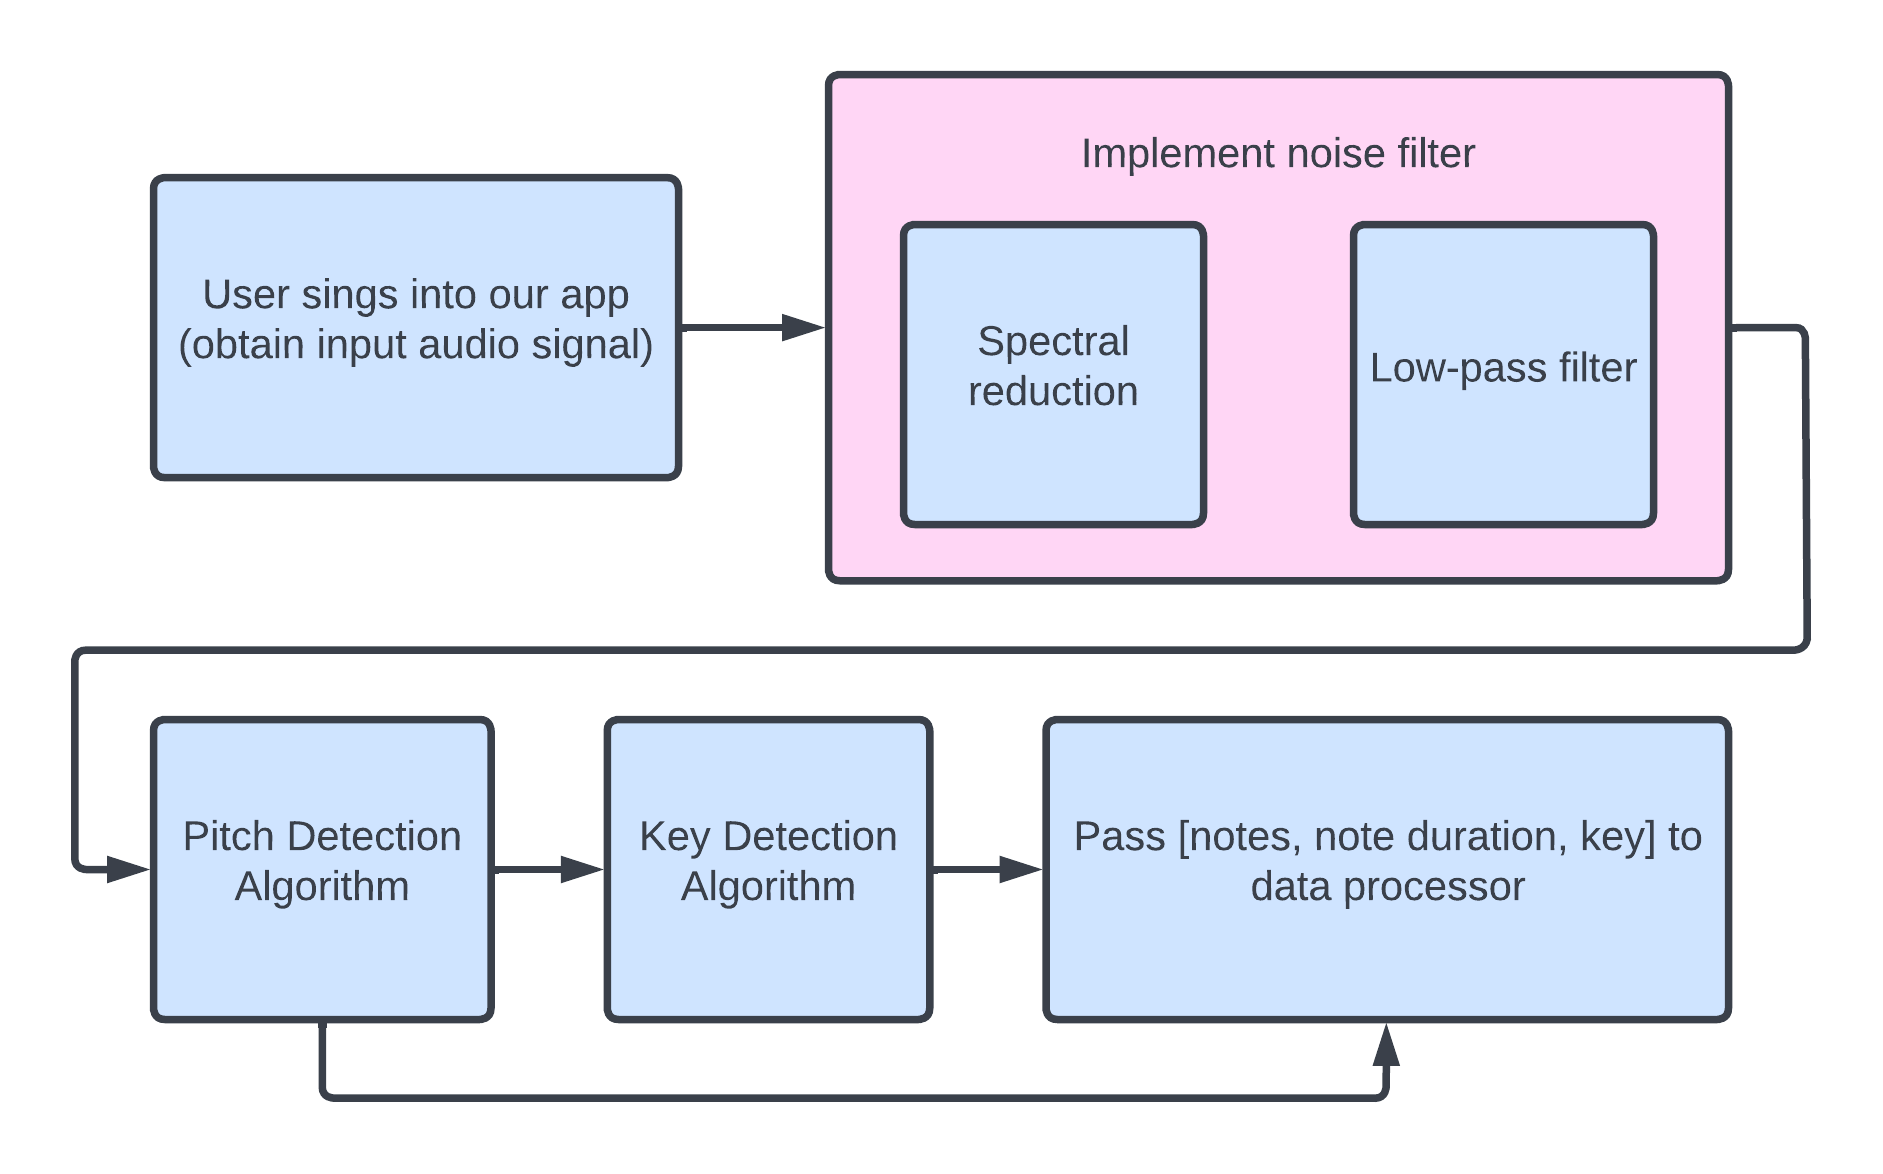
\includegraphics[width=0.8\columnwidth]{Figures/Audio Processing Flow Chart}
    \decoRule
    \caption{Flowchart of audio processing}
    \label{flowchart}
\end{figure}
%----------------------------------------------------------------------------------------
%   SECTION 0
%----------------------------------------------------------------------------------------
\section{Assumptions}
\label{sec:asm}
Before we delineate the approach to audio processing, there are some assumptions that our model
is built on:

\begin{assumption}\label{as:1}
    Users' audio input device does not contain active noise cancelling functions.
\end{assumption}

\begin{assumption}\label{as:2}
    Signal and noise are uncorrelated.
\end{assumption}

\begin{assumption}\label{as:3}
    Noise is a stationary or slowly varying process, i.e. noise spectrum does not change drastically during the recording.
\end{assumption}

\begin{assumption}\label{as:4}
    Users do not sing with the technique of polyphonic overtone singing.
\end{assumption}

\begin{assumption}\label{as:5}
    Users only sing in major keys.
\end{assumption}

They will be referred to and explained in the later sections.

%----------------------------------------------------------------------------------------
%   SECTION 1
%----------------------------------------------------------------------------------------
\section{Noise Filter}
\label{sec:NF}
Noise filtering is essential as it reduces or eliminates the noise present in the input signal.
A conventional method to quantify noise is the signal-to-noise ratio (SNR), which is often 
represented in decibels.
\[SNR=10*log_{10}\frac{P_{signal}}{P_{noise}}\]
As its name suggests, SNR is the power ratio between the desired signal and undesired noise. Effectively,
we would like to use noise filters to achieve a higher SNR.\\ 
There are a few noise sources when a user records himself with a microphone.
Firstly, self-noise exists, which is the instrument noise produced by the microphone itself.
Noise may be induced or created when the signal passes through electronic components like transistors 
and printed circuit boards\footnote{Arthur. (October 2018). What is microphone self-noise? (equivalent noise level). My New Microphone. Retrieved May 15, 2022, from https://mynewmicrophone.com/self-noise/ }.
The second source, ambient noise, contributes to a large portion of noise present in a recording.
Room reflections, extraneous noise, electromagnetic interference and mechanical noise are some ambient noise causes.  

%-----------------------------------
%   SUBSECTION 1
%-----------------------------------
\subsection{Possible Models}
Most of the noise filters work in the frequency and spectral-domain here. We are going to inspect and
compare three noise reduction mechanisms.

\begin{enumerate}
    \item \textbf{Low-pass filter (LPF)}\\
    LPF passes signals with frequency \(f<f_{c}\), where \(f_{c}\) is the cut-off frequency, and attenuates
    signals with \(f>f_{c}\). 
    In order to implement an LPF, we have to transform the signal from time domain to 
    frequency domain using Fourier Transform (FT). An ideal LPF would completely remove frequencies that are
    higher than \(f_{c}\) and is a non-casual linear time-invariant system. 
    \[H(f) = rect(\frac{f}{2B})\]
    \[h(t))= \mathfrak{F}^{-1}{H(f)} = \int_{-B}^{B} e^{2(\pi)ift}\,df = 2Bsinc(2Bt)\]
    The impulse response of an LPF is a sinc function that extends to [-$\infty$,$\infty$]. This is why it is 
    impossible to realize an ideal LPF since that will take infinite time and memory.

    \item \textbf{Wavelet transform}\\
    Wavelet transform creates a representation of the signal in both the time and frequency domain so localised 
    signal information can be efficiently accessed. It is often compared with FT, which
    has the following limitations: 
    \begin{enumerate}
        \item For windowed FT, if the feature is larger or shorter than the window, it cannot be captured completely.
        \item Time resolution for high frequencies is the same for low frequencies. As frequency increases, the rate of 
        change of the signal increases, and high-frequency signals contain more information in a window than that of 
        low frequency. Thus we need a higher time resolution for that.
    \end{enumerate}
    Wavelet transform analyses a signal by its different frequency components at multiple resolutions, so features that are 
    undiscovered at one resolution may be evident at another. There are mainly two types of wavelet transforms: continuous wavelet transform (CWT) and discrete wavelet transform (DWT).
    
    CWT finds how alike a wavelet is in a signal, given the dilation and translation parameter of the wavelet\footnote{Talebi, S., Contributor, E., \&; Shawhin Talebi is a Physics PhD\&;candidate at the University of Texas at Dallas. (n.d.). Fourier vs. wavelet transform: What's the difference? Built In. Retrieved May 15, 2022, from https://builtin.com/data-science/wavelet-transform }.
    This can be found by convolving the mother wavelet with our signal.

    \begin{equation*} 
        \text{CWT}(\mathrm{a},\mathrm{b}; \mathrm{x}(\mathrm{t}),\psi(\mathrm{t}))=\int_{-\infty}^{\infty}[\mathrm{x}(\mathrm{t})\frac{1}{\mathrm{a}}-\psi^{*}(\frac{\mathrm{t}-\mathrm{b}}{\mathrm{a}})]\text{dt}
    \end{equation*}

    where \(x(t)\) is the original signal, \(\psi(t)\) is the mother wavelet, \(a\) is a dilation parameter and \(b\) is a translation parameter \footnote{Dautov, Çiğdem Polat and Özerdem, Mehmet Siraç. (2018). Wavelet transform and signal denoising using Wavelet method. In 2018 26th Signal Processing and Communications Applications Conference (SIU) (pp. 1–4). essay. }.
    The dilation factor represents how dispersed the wavelet is (similar to scaling), while the translation factor tells us where the wavelet is
    positioned in time (similar to shifting). 
    
    \begin{figure}
        \centering
        \begin{subfigure}{.4\textwidth}
          \centering
          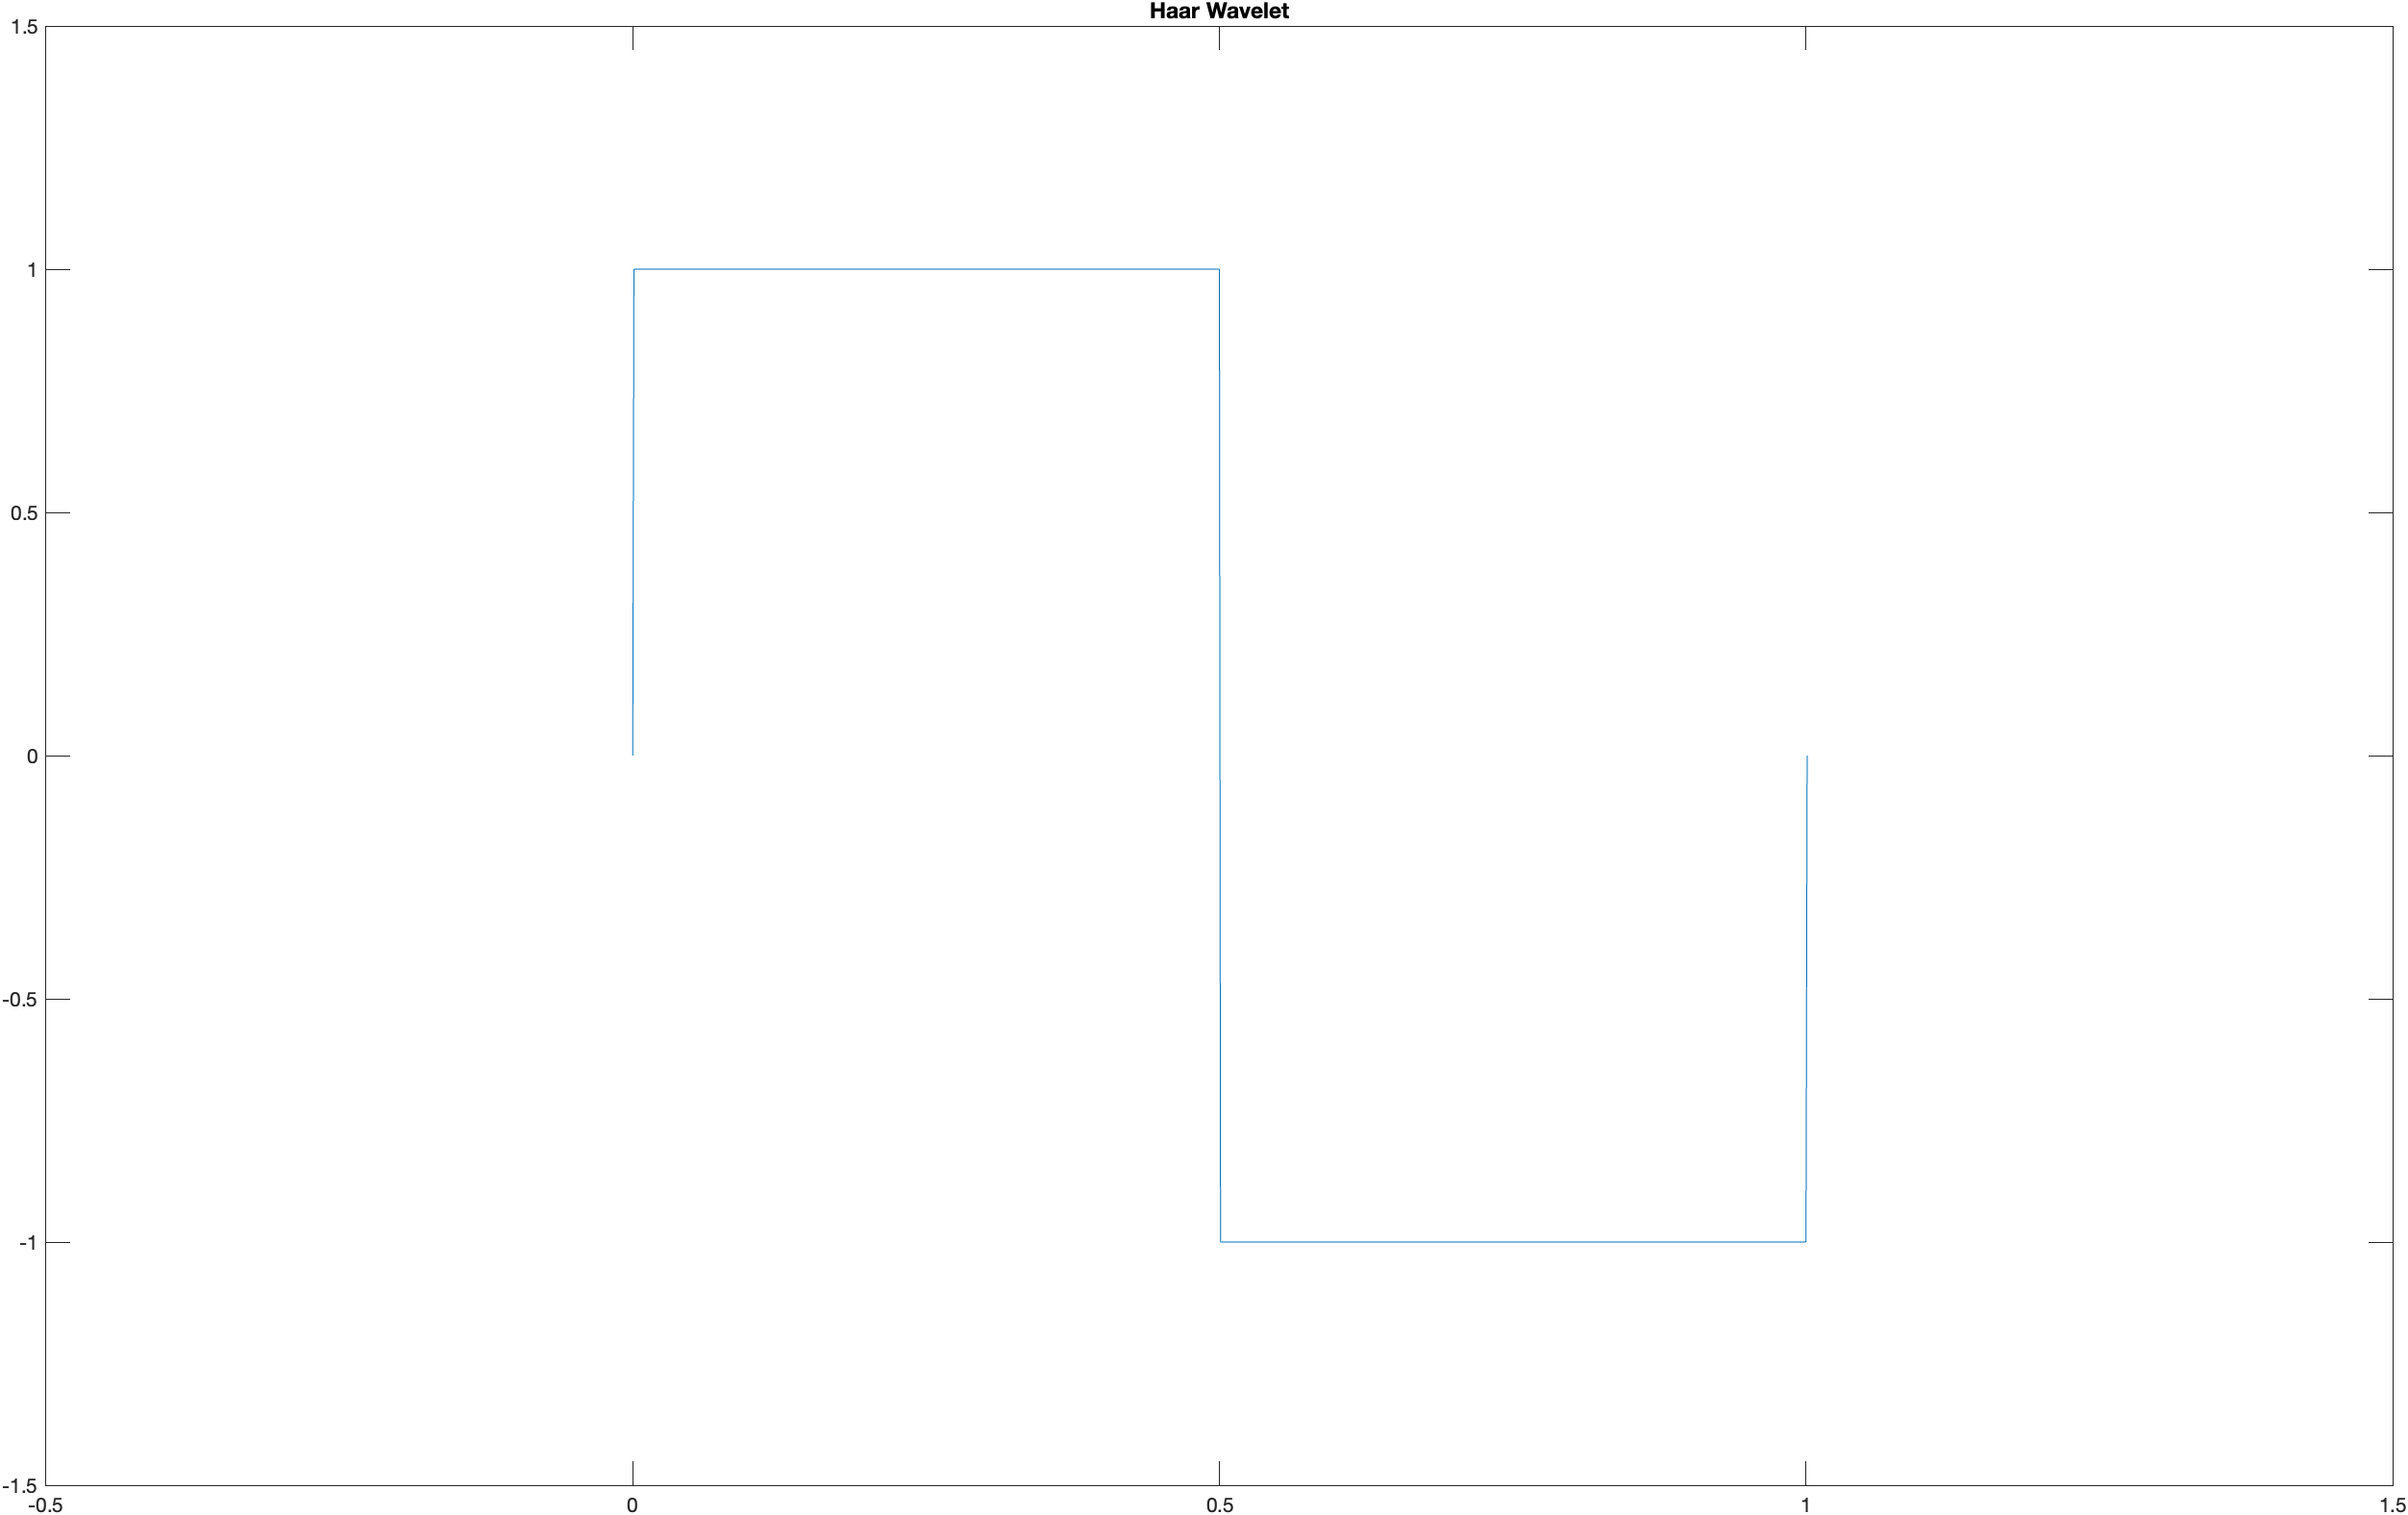
\includegraphics[width=\linewidth]{Figures/haar.png}
          \caption{Haar wavelet}
          \label{Haar}
        \end{subfigure}
        \hfill
        \begin{subfigure}{.4\textwidth}
            \centering
            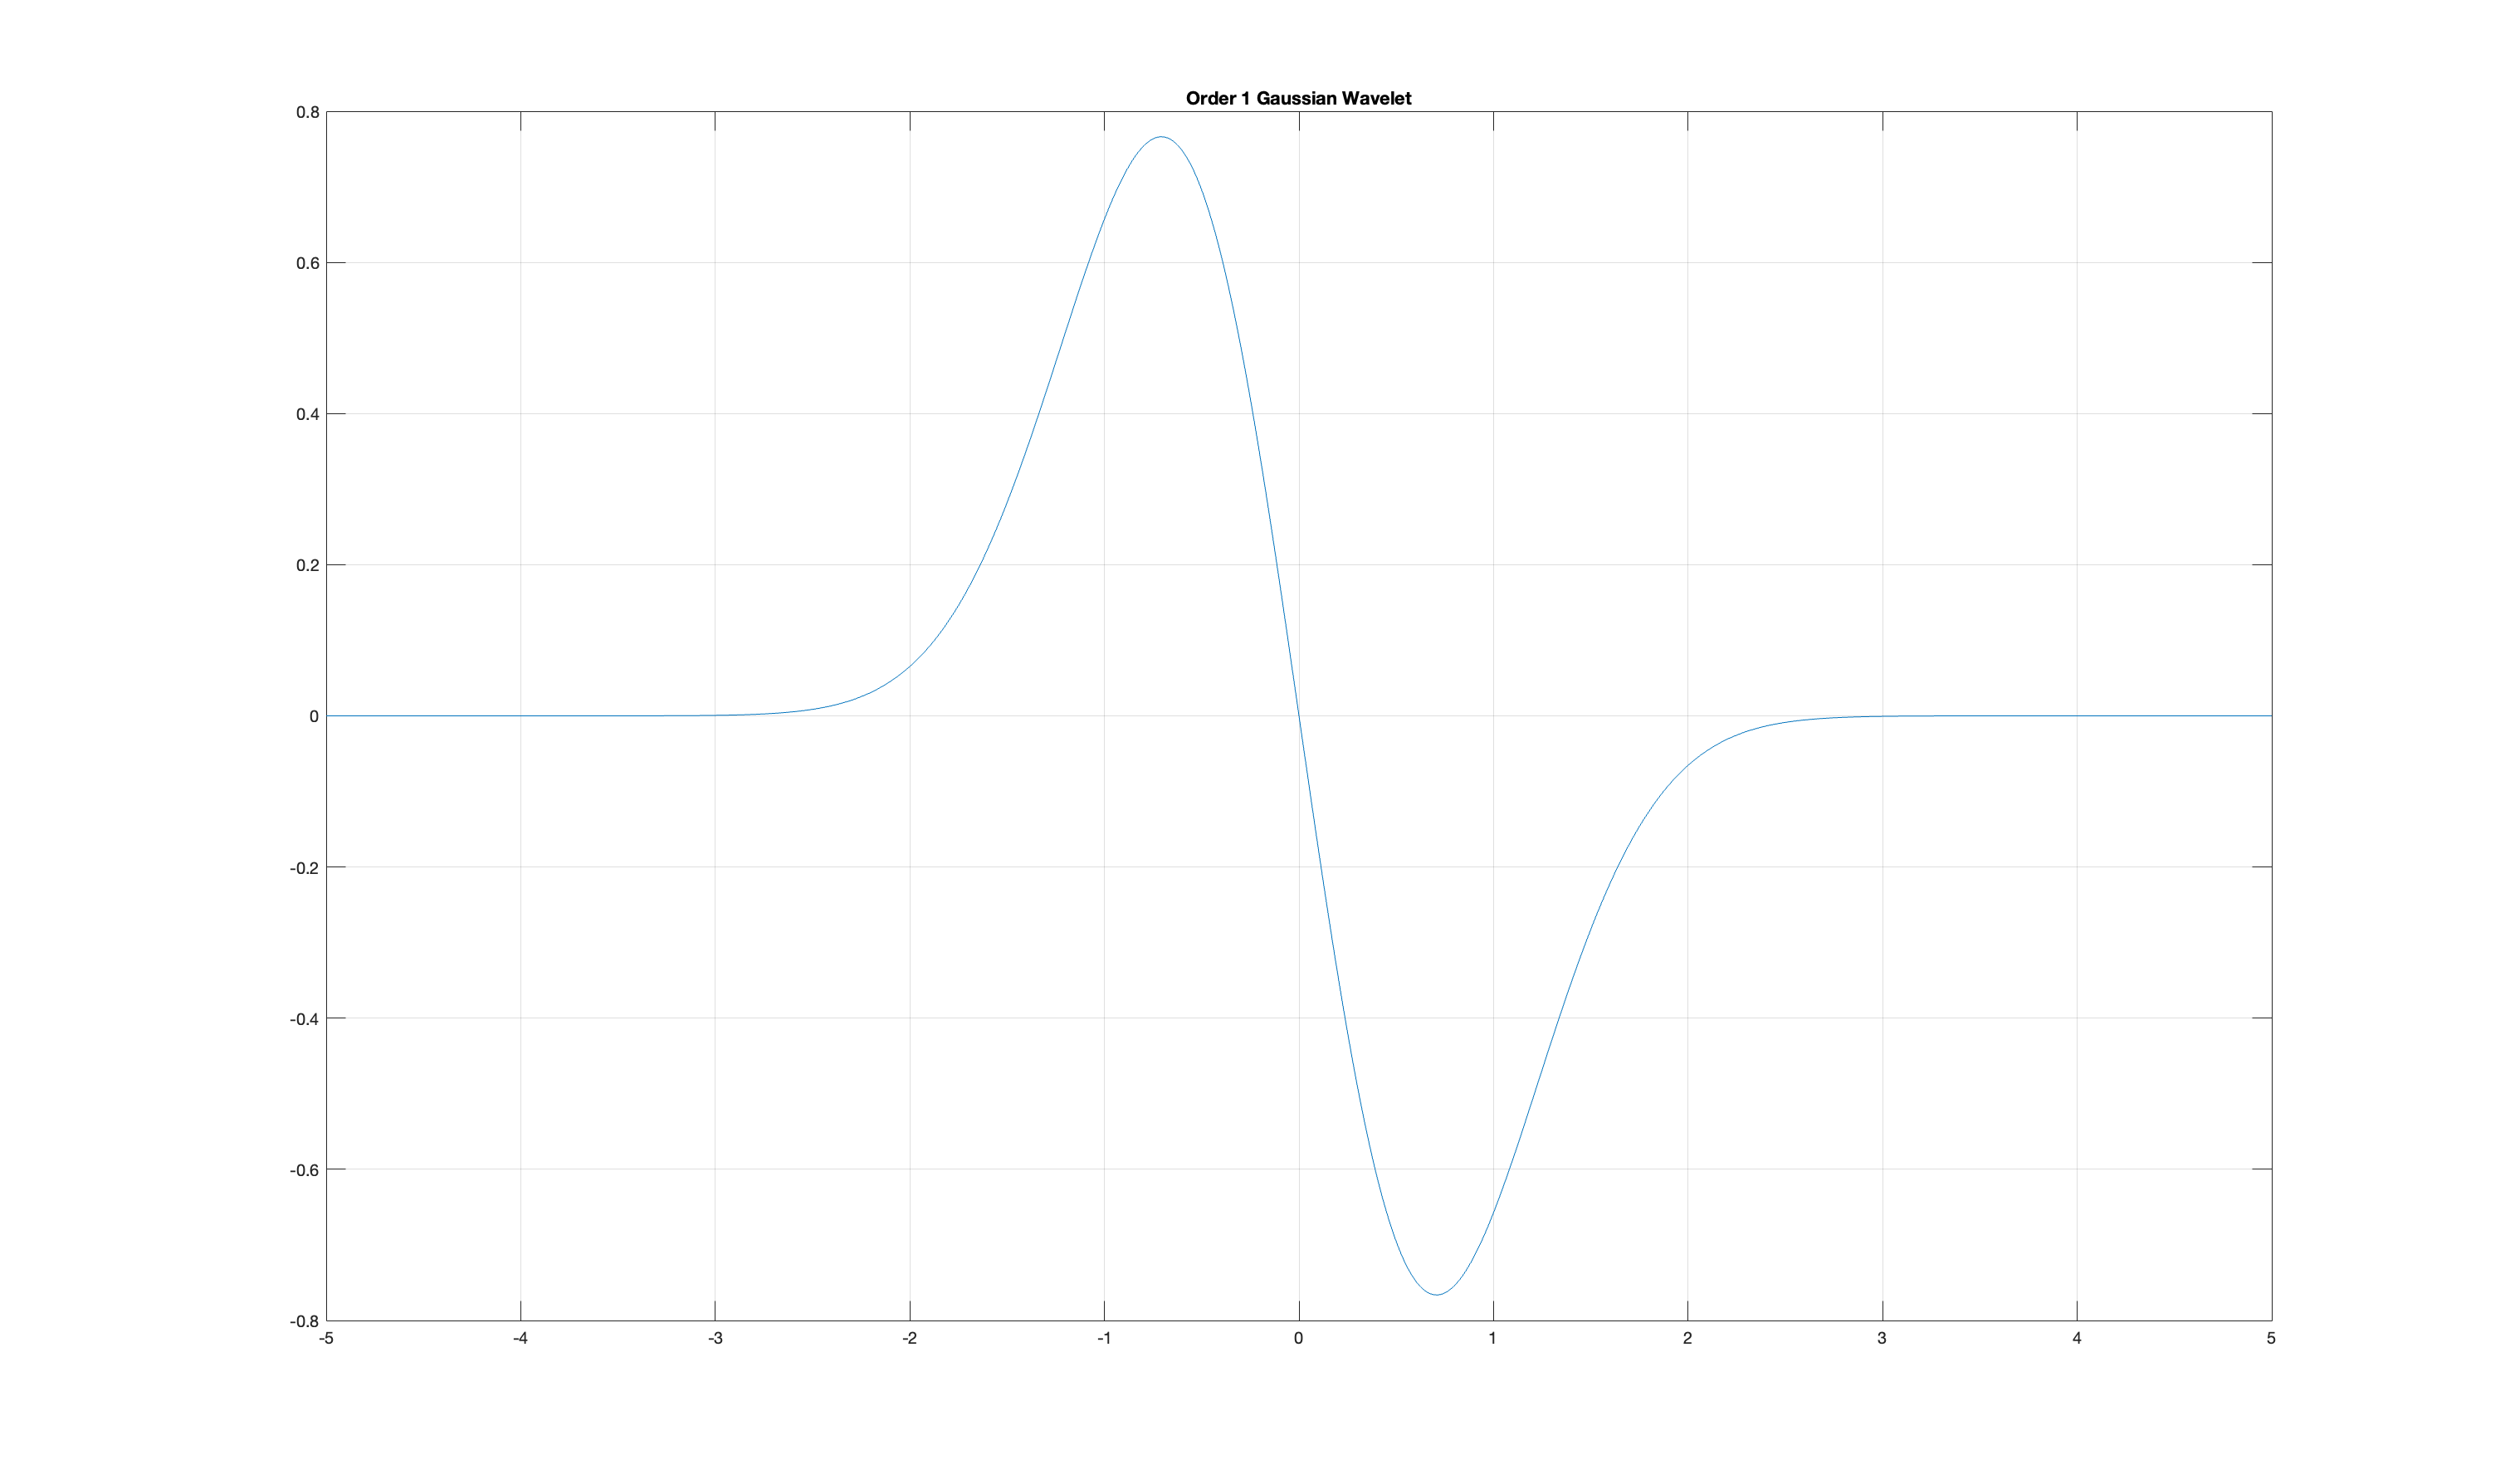
\includegraphics[width=\linewidth]{Figures/order1gaussian.png}
            \caption{Gaussian wavelet \\of order 1}
            \label{order1}
        \end{subfigure}
        \hfill
        \begin{subfigure}{.4\textwidth}
          \centering
          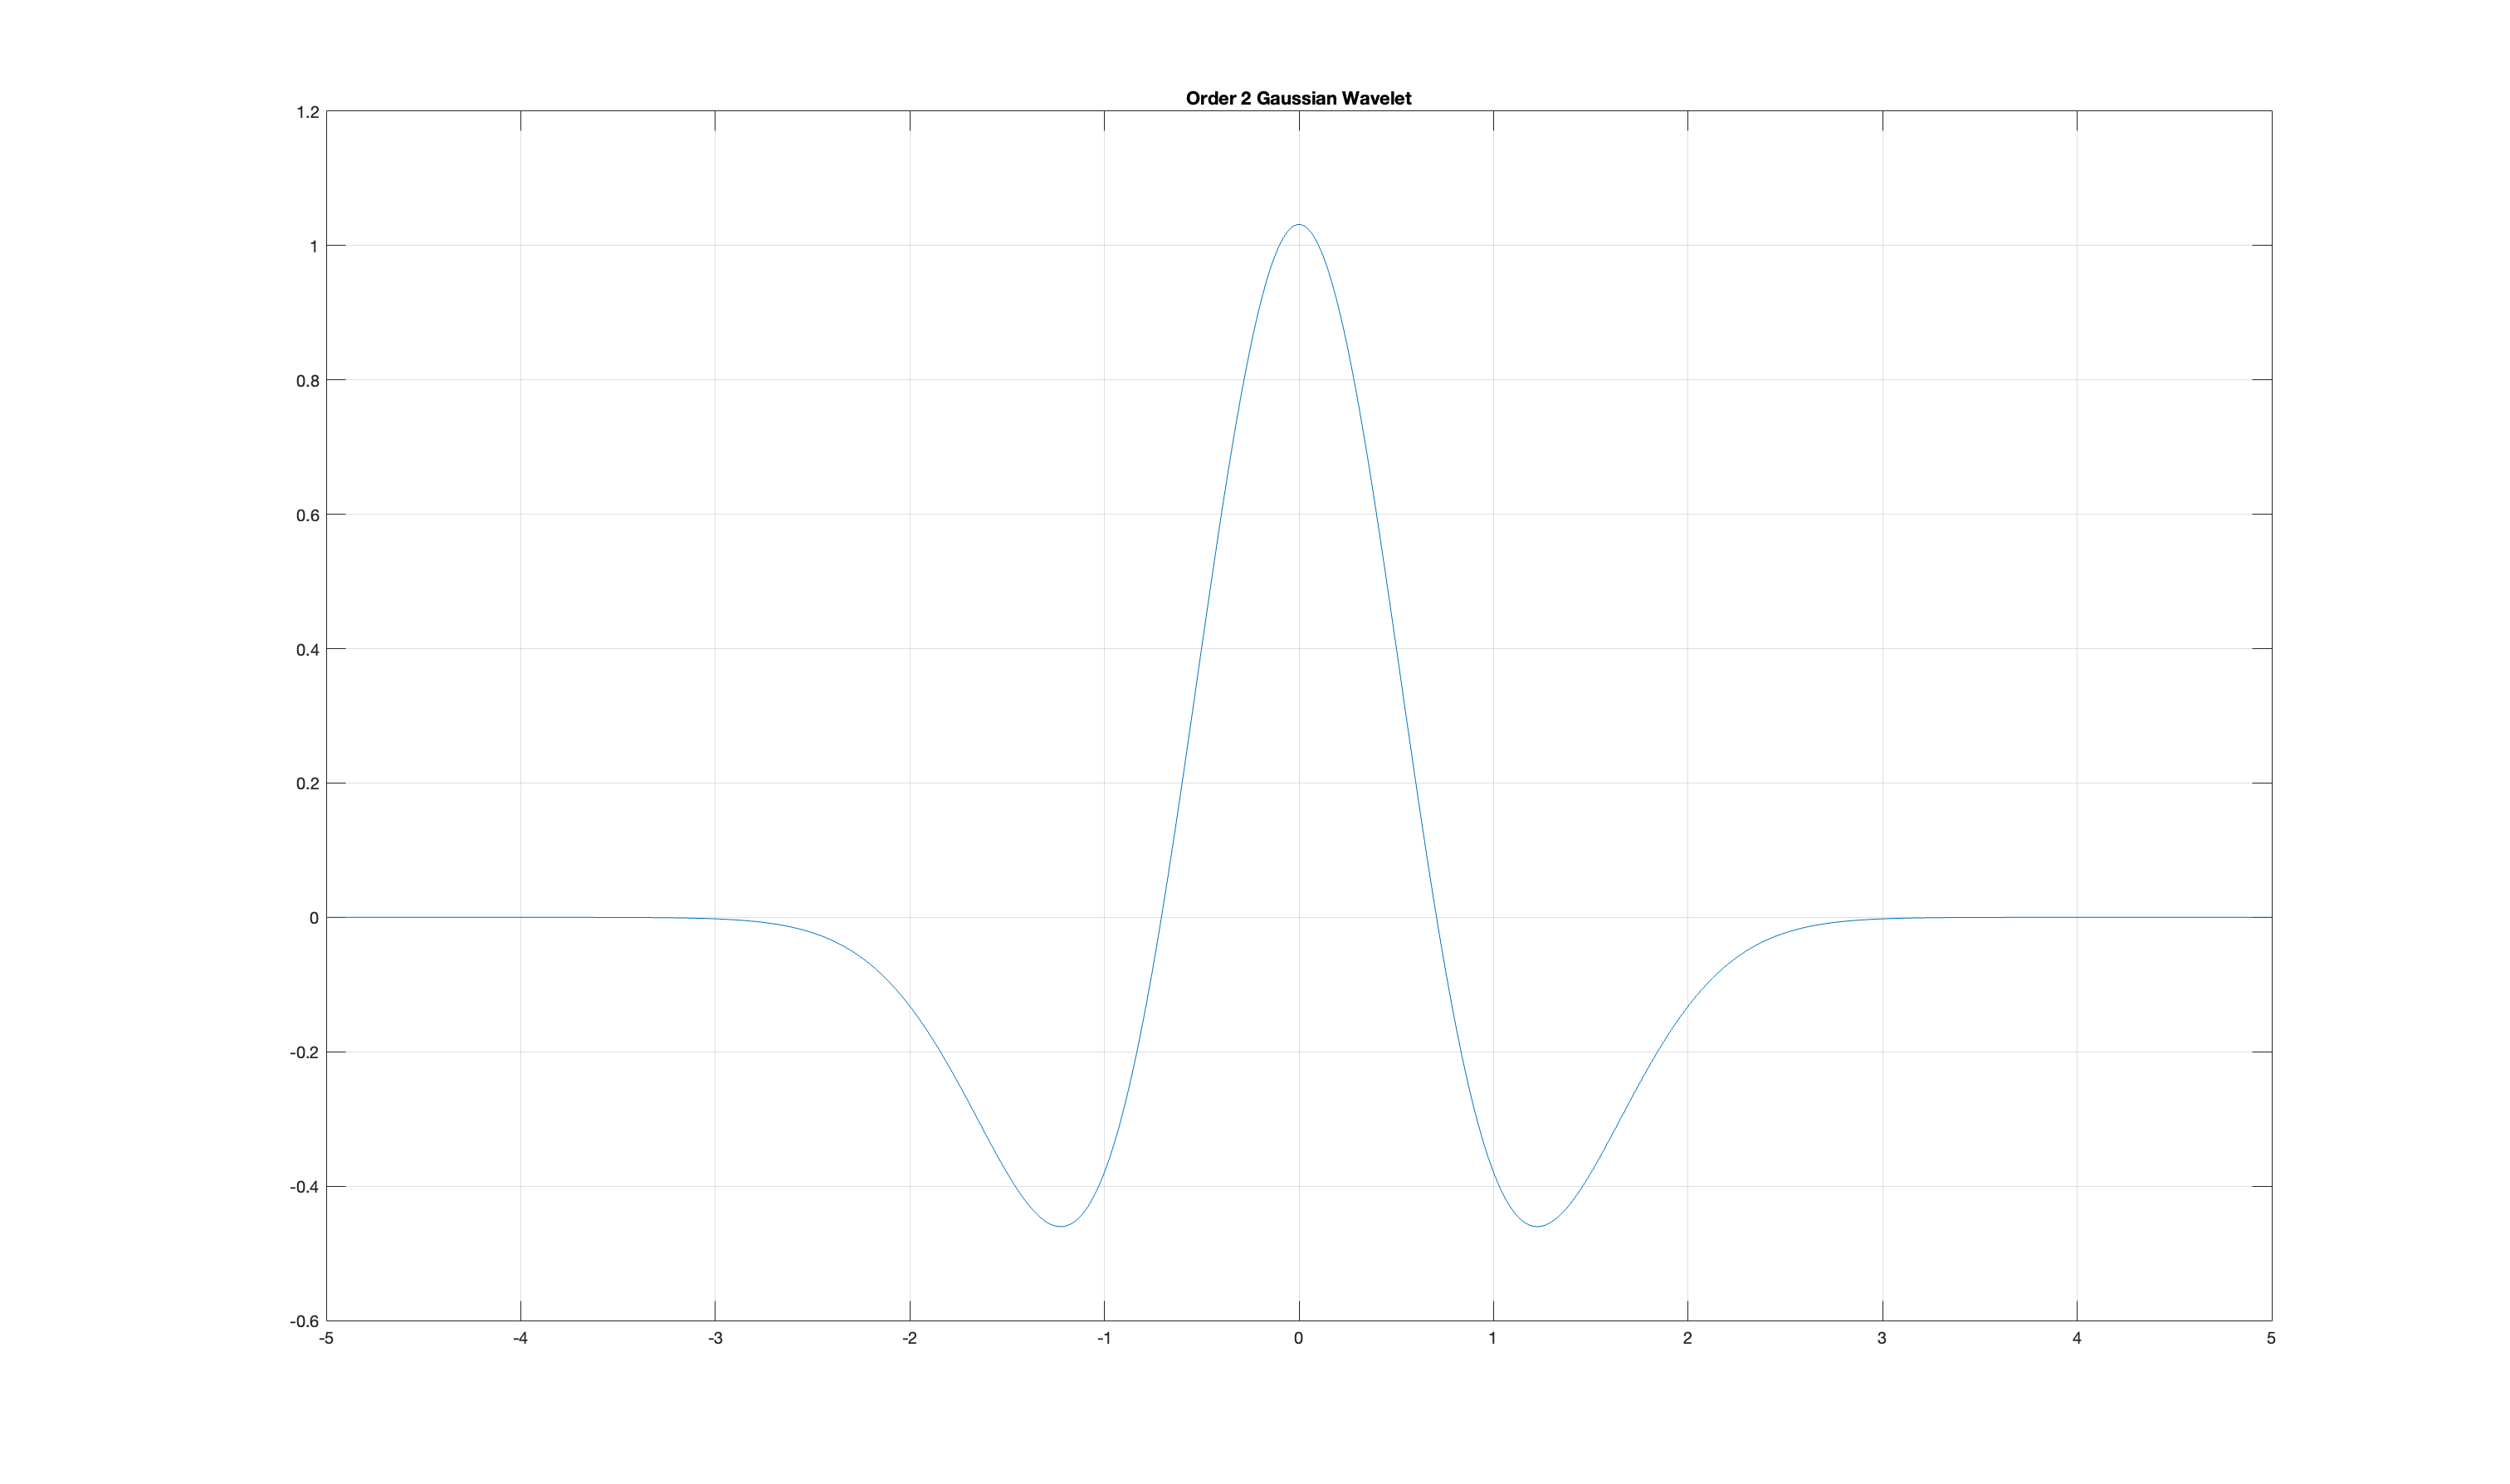
\includegraphics[width=\linewidth]{Figures/order2gaussian.png}
          \caption{Ricker wavelet - Gaussian \\wavelet of order 2}
          \label{Ricker}
        \end{subfigure}

        \caption{Examples of wavelets}
        \label{fig:test}
    \end{figure}
    
    The major difference between DWT and CWT is how the scale parameter is discretized. DWT discretizes scale parameters to integer power of 2 while CWT is more refined since 
    the scale parameter is often raised to different fractional powers.
    \begin{align*} &\text{DWT}\ [\mathrm{n},\mathrm{a}^{\mathrm{j}}]=\sum_{\mathrm{m}=0}^{\mathrm{N}-1}\mathrm{x}[\mathrm{m}].{\psi_{\mathrm{j}}}^{*}[\mathrm{m}-\mathrm{n}],\\ &\psi_{\mathrm{j}}[\mathrm{n}]=\frac{1}{\sqrt{\mathrm{a}^{\mathrm{f}}}}\psi\left(\frac{\mathrm{n}}{\mathrm{a}^{\mathrm{f}}}\right) \tag{2} \end{align*}
    where \(n\) is delay parameter, \(N\) is the length of signal, \(\psi\) is the discretized mother wavelet. 

    DWT is often preferred in the context of real-time audio processing since computation is done on discrete wavelets, which require less computational resources.
    
    \item \textbf{Spectral reduction}\\
    Spectral noise gating learns from a noise profile and removes the signal's slow-changing tonal noise or hiss. Audacity uses this method in its noise reduction algorithm \footnote{How audacity noise reduction works. How Audacity Noise Reduction Works \- Audacity Wiki. (n.d.). Retrieved May 15, 2022, from https://wiki.audacityteam.org/wiki/How\_Audacity\_Noise\_Reduction\_Works}.
    Suppose noise is additive, and we can represent our noisy audio as
    \begin{align}\label{sreduction} 
    y(n) = x(n) + d(n), \text{ for } 0 \leq n \leq N-1 
    \end{align}
    where $x(n)$ is our original signal (the signal we wish to recover), $d(n)$ is the noise, $n$ is the discrete time index,
    $N$ is the number of samples. 
    Assuming $d(n)$ and $x(n)$ have no correlation (\cref{as:2}), and we perform a short-time fourier transform on equation \cref{sreduction}:
    \[Y(\omega,k)= X(\omega,k) + D(\omega,k)\]
    where $k$ is the frame number. Each frame will be of
    length $N$. We then have the desired signal in frequency domain:
    \[X(\omega,k) = Y(\omega,k) - N(\omega,k)\]
    Since the statistics of the noise is unknown, we try to find an estimate of noise spectrum by calculating the time-averaged
    noise spectrum using parts of the recording that only contain ambient noise\footnote{Multimedia Systems Department, Gdansk University of Technology and Air Force Academy in Deblin. (2004). Noise Reduction. Noise reduction. Retrieved May 15, 2022, from https://sound.eti.pg.gda.pl/denoise/noise.html}.
    \begin{align} 
    \hat{N}(\omega,k) = \textbf{E}[|N(\omega,k)|] = \frac{1}{N}\sum_{i=0}^{N-1}|N_i(\omega,k)|
    \end{align}
    We then get the estimated signal spectrum
    \begin{align}
    \hat{X}(\omega,k) = Y(\omega,k) - \hat{N}(\omega,k)
    \end{align}
    We then set a gain control for each frequency band, so if the sound exceeds the threshold, the gain is set to 0 dB or a user-defined
    constant.
\end{enumerate}
%-----------------------------------
%   SUBSECTION 2
%-----------------------------------
\subsection{Choice of model and implementation}
After trying to implement all three methods, a significant difficulty encountered is that it is hard to set the parameters to 
implement for LPF and wavelet transform.
For example, since $f_c$ depends on the pitch range of the user and the melody they are inputting, finding an adequate $f_c$ that separates desired frequencies from undesired ones is hard.
As for wavelet transform, finding a proper mother wavelet is a difficult task.
Although wavelet transform works better for real-life non-stationary signals compared to conventional frequency-based filters, if we
do not feed a suitable mother wavelet, the performance is unsatisfactory, the model cannot distinguish between desired and undesired 
signals and will decrease $P_{signal}$ at the same time, which is unfavourable when it comes to improving the SNR.
According to \cite{complexwt}, there are two major concerns with using wavelet transform. 
Firstly, it is sensitive to shifts in time; even a minor shift will cause an unpredictable change in transform coefficients which will 
then cause variations in the output signal. Secondly, wavelet transform suffers from poor directionality easily. For example, 
a 2-D DWT can only reveal three spatial-domain feature orientations, limiting the signal's optimal representation. 

Therefore, we decided to use spectral reduction as our noise filter algorithm since it is the most effective in removing the ambient noise 
and wideband noise. Note that this method heavily assumes that the noise spectrum magnitude is staying locally 
stationary \autoref{as:3}. If this assumption is not satisfied, this method will result in poor performance of either not being able to filter
 a majority of the broadband noise or removing the features of the signal.
The implementation of spectral noise gating can be summarised according to \cite{spectralflowchart} as shown in \cref{spectralflowchart}
\begin{figure}
	\centering
	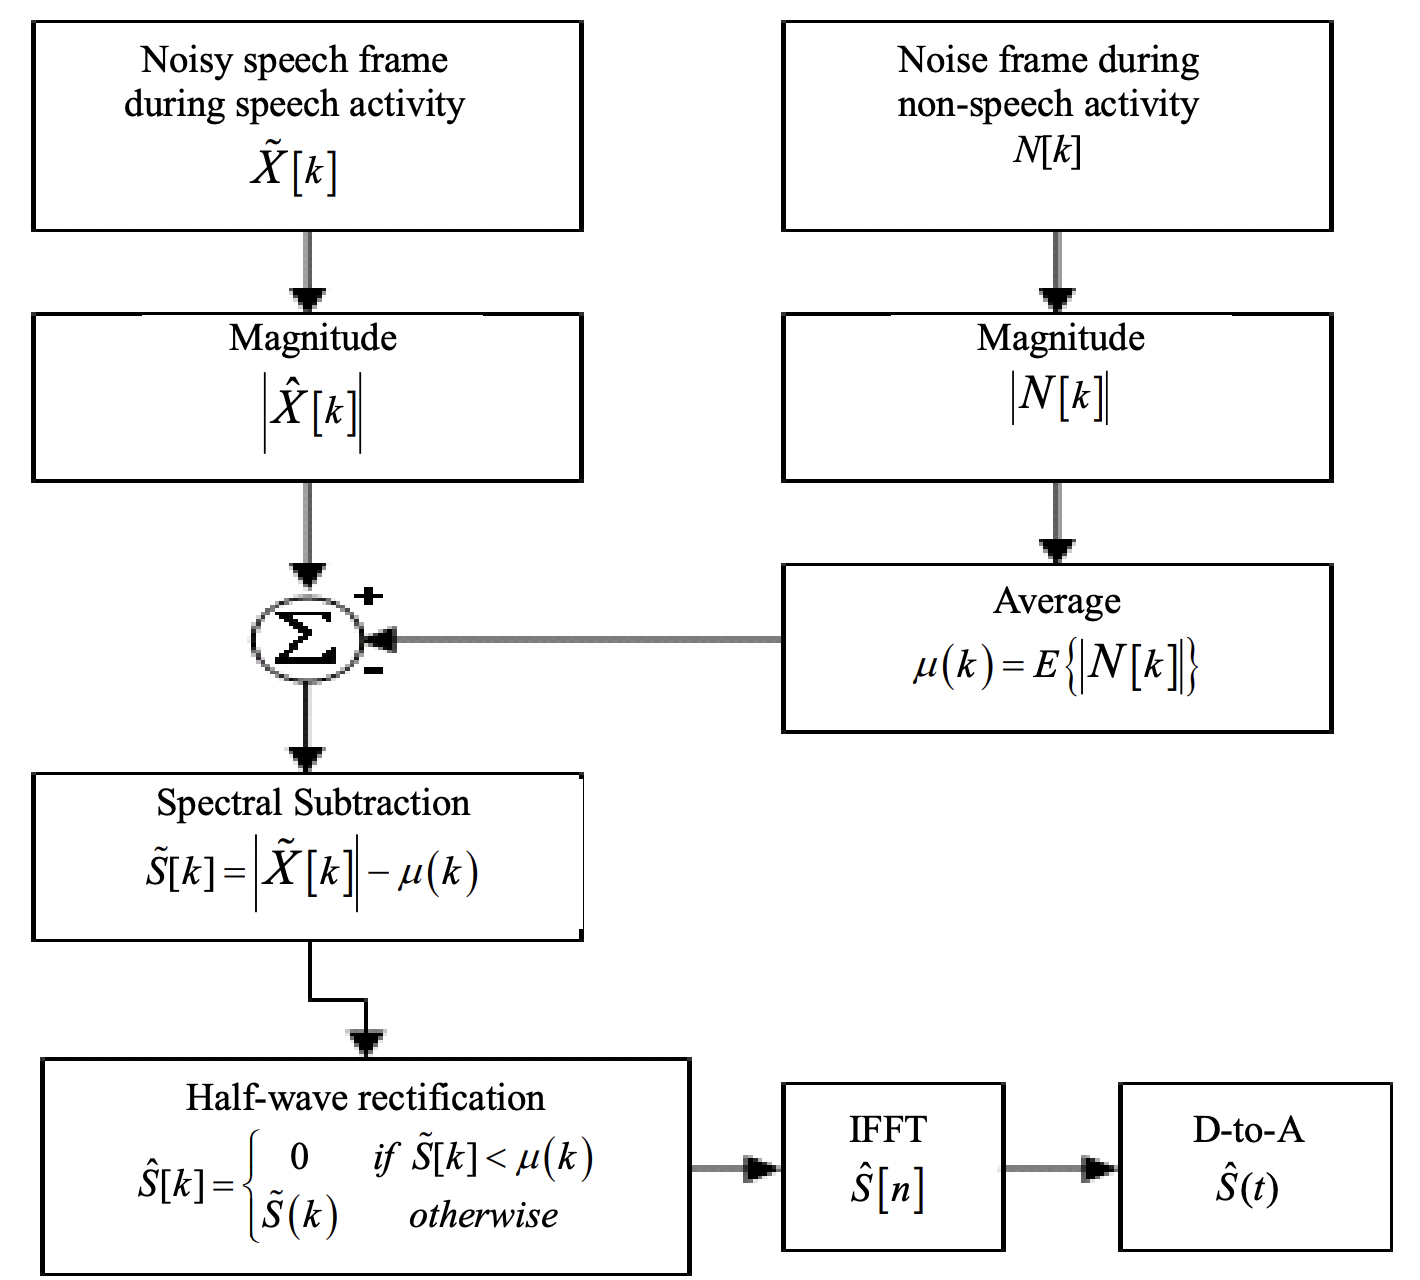
\includegraphics[scale=0.35]{Figures/spectralprocess.png}
	\caption{Spectral noise gating flowchart}
	\label{spectralflowchart}
\end{figure}
The noise spectrum $N(\omega,k)$ and its statistical measures are obtained by asking users to record at least 3 seconds of silence 
before they sing into the app.

Note that half-wave rectification is necessary after the noise removal process of subtracting the average magnitude of the noise spectrum. 
\begin{equation}
    \abs{\hat{X}(\omega,k)} = \begin{cases}
        \abs{\hat{X}(\omega,k)}   & \text{if } \hat{X}(\omega,k) \leq 0\\
        0                     & \text{otherwise.}
    \end{cases}
\end{equation}

This is to target frequencies that have a higher average magnitude of noise spectrum $\textbf{E}[|N(\omega,k)|]$ compared to that of 
the noisy speech spectrum $|\hat{X}(\omega,k)|$. For those frequencies, we would replace the negative values with 0 with a half-wave 
rectification.

Referring back to \autoref{as:1}, it is prime to require our users not to use any active noise-cancelling inputs since the spectral reduction
the method may not function accurately since the noise amplitudes get attenuated.

%-----------------------------------
%   SUBSECTION 3
%-----------------------------------
\subsection{Improvements}
A drawback of spectral reduction is that it does not nicely handle extreme responses. It does not reduce noises like
squeaks. Also, since a half-wave rectification is included in the implementation process, \cite{spectral_drawback} has 
pointed out that residual noise will be created during the process of spectral reduction. Half-wave rectification introduces
nonlinearity in the $\hat{X}(\omega,k)$ spectrum and results in frequencies changing abruptly between frames.

To reduce the residual noise, we can modify the rectification so that when the estimated 
signal spectrum is negative (i.e. when the magnitude of noise spectrum is larger than that of the 
noisy signal spectrum), we use the noisy signal spectrum magnitude.
\begin{equation}
    \abs{\hat{X}(\omega,k)} = \begin{cases}
        \abs{\hat{X}(\omega,k)}   & \text{if } \hat{X}(\omega,k) \leq 0\\
        \abs{Y(\omega,k)}                   & \text{otherwise.}
    \end{cases}
\end{equation}

On the other hand, as mentioned above, the spectral reduction is built on the assumption that the noise is stationary or slowly varying. Yet, in reality,
sudden squeaky noise in the background may not be recorded in the noise profile. In this case, the spectral reduction 
cannot remove the squeak. We will introduce a low-pass filter to filter out high-frequency noise to improve the situation. The reason
for choosing LPF over a bandpass filter is that spectral reduction effectively targets the reduction of ambient noise, which is
 usually low frequency. Thus, to avoid removing low-frequency desirable features, a low-pass filter will suffice.

To determine $f_c$ for the LPF, it would be plausible to refer to the biological features of the users, i.e. their age and gender.
For males, the pitch level generally reduces from infancy to middle age, while the trend reverses after middle age. 
On the other hand, as pointed out by \cite{womenprange}, "Females in their 30s and 40s showed lower frequencies than those in their
20s. Across all age groups, including the 80s, fundamental frequencies tended to decrease markedly in association with aging”


\begin{figure}
    \CenterFloatBoxes
    \begin{floatrow}
        \ffigbox{
            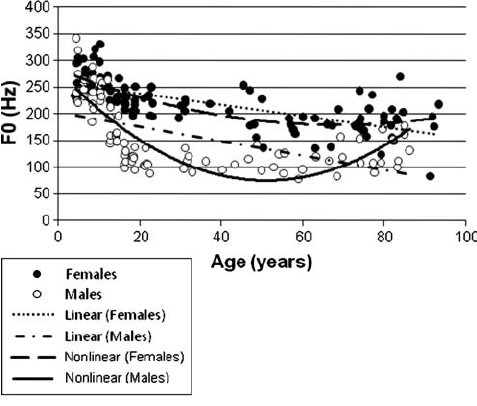
\includegraphics[scale=0.4]{Figures/f0vage.jpeg}
            }{
            \label{f0vage_chart}
		    \caption{Scatter plot of\\fundamental frequency}
        }
        \killfloatstyle
        \ttabbox
            {\begin{tabular}{lrr}		& Male   & Female  \\
			    Pitch range (Hz)            & 60-180 & 160-300 \\
			    Praat pitch range (Hz) 		& 50-300 & 100-600
		    \end{tabular}
            }{
            \label{table:praat}
            \caption{Praat pitch range }
            }
    \end{floatrow}
\end{figure}

After referring to the measurements taken from 192 participants\footnote{Stathopoulos, E. T., Huber, J. E., \&; Sussman, J. E. (2011). Changes in acoustic characteristics of the voice across the life span. Journal of Speech, Language, and Hearing Research, 54(4). https://doi.org/10.1044/1092-4388(2010/10-0036) } 
and the pitch range set by Praat
\footnote{Goldstein, Louis. (n.d.). Measuring F0 Contours using Praat: Configuring the pitch contour. Retrieved May 15, 2022, from https://www.fon.hum.uva.nl/praat/manual/Intro\_4\_2\_Configuring\_the\_pitch\_contour.html} 
(a software for speech analysis), a simple modelling of $f_c$ according to age and gender is as below:
\[f_{c,male}(n) = 0.07n^2 - 7.5n + 480, \text{ for } 4 \leq n\leq 93 \label{male} \] 
\[f_{c,female}(n) = 0.02n^2 - 3n + 687, \text{ for } 4 \leq n \leq 93 \label{female} \] 
where $n$ is the age of the user.
In deciding which filter to implement, there are 3 filters in consideration:
\begin{enumerate}[label=(\alph*)]
    \item Type 1 Chebyshev filter
    \[G_{n}(\omega) = |H_{n}(j\omega)| = {\frac{1}{\sqrt{1+\varepsilon^{2} T_{n}^{2}(\frac{\omega}{\omega_{0}})}}}\]
    where $\varepsilon$  is the ripple factor, $\omega _{0}$ is the cut-off frequency
    and $T_{n}$ is a Chebyshev polynomial of the $n$th order.
    \item Butterworth filter
    \[G_{n}(\omega) = |H_{n}(j\omega)| = {\frac{1}{\sqrt{1+(\frac{\omega}{\omega_{0}})^{2n}}}}\]
    where $\omega _{0}$ is the cut-off frequency and $n$ is the order of filter.
    \item Bessel filter
    \[G_{n}(\omega) = |H_{n}(j\omega)| ={\frac {\theta _{n}(0)}{\theta _{n}(\frac{j\omega}{\omega _{0}})}}\]
    where $\theta _{n}(j\omega)$ is a reverse Bessel polynomial and $\omega _{0}$ is the cut-off frequnecy
\end{enumerate}

Chebyshev filter has a steeper roll-off than Butterworth and Bessel filter. Still, it also brings passband and stopband ripples, 
unlike Butterworth and Bessel filters, which have a flat passband and stopband as they roll off towards zero. Moreover, Butterworth 
and Bessel's filters have a better step response. Meanwhile, Bessel filters perform the best in step response since the overshoot is
minimal. Another benefit the Bessel filter has is it introduces a linear phase and constant delay for $f<f_c$. This
feature allows us to preserve the waveshape since the same amount delays all frequencies.
Thus, a Bessel filter is preferred in this context.

\begin{figure}[h]
	\centering
	\begin{subfigure}{.4\textwidth}
	  	\centering
	  	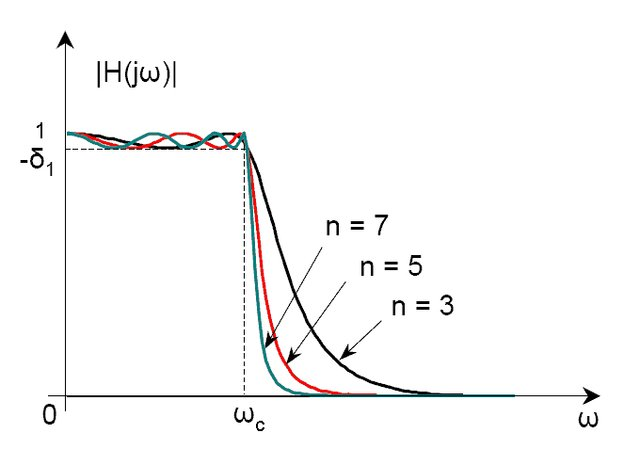
\includegraphics[width=1\linewidth]{Figures/chebyshev.jpeg}
	  	\caption{Type 1 Chebyshev filter \\frequency response}
	  	\label{fig:sub1}
	\end{subfigure}
	\hfill
	\begin{subfigure}{.4\textwidth}
	  	\centering
	  	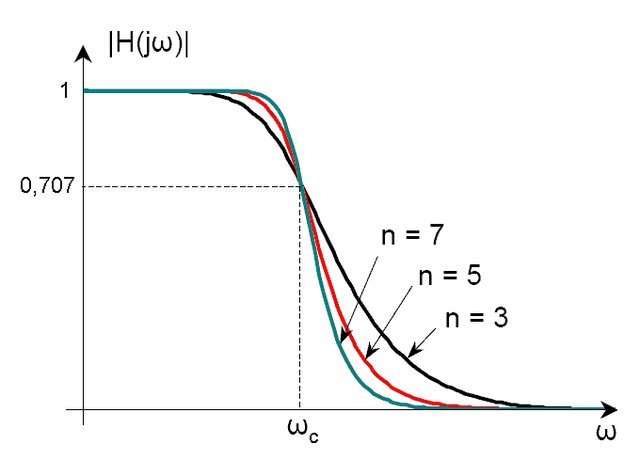
\includegraphics[width=1\linewidth]{Figures/butterworth.jpeg}
	  	\caption{Butterworth filter frequency response}
	  	\label{fig:sub2}
	\end{subfigure}
	\hfill
	\begin{subfigure}{.4\textwidth}
		\centering
		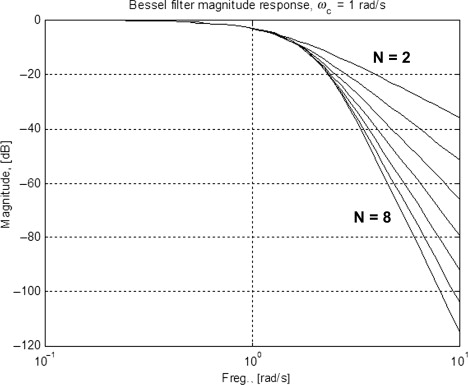
\includegraphics[width=1\linewidth]{Figures/bessel.jpg}
		\caption{Bessel filter frequency\\response}
		\label{fig:sub3}
	\end{subfigure}

\end{figure}

%----------------------------------------------------------------------------------------
%   SECTION 2
%----------------------------------------------------------------------------------------
\section{Pitch Detection Algorithm (PDA)}
\label{sec:PDA}
After removing noise, we pass the processed signal to a PDA to estimate the fundamental frequency ($f_0$) of
the signal. Before we explain the algorithm, we would assume that our users will not input polyphonic overtone 
singing \autoref{as:4}, i.e. creates notes of multiple fundamental frequencies at the same time, since the technique is uncommon
. It requires further investigation on building a robust PDA that can identify different notes at one time period.

%-----------------------------------
%   SUBSECTION 1
%-----------------------------------
\subsection{Possible Models}
There are four approaches to detect $f_0$, which can be classified into the time domain and frequency domain.

\begin{enumerate}
    \item \textbf{Zero crossings (time domain)}\\
    This is the most intuitive method to detecting pitch although it suffers from low accuracy.
    Assuming the input is monophonic, the fundamental frequency is estimated as:
    \[f_0 = \frac{P_{zcr}f_s}{2N}\]
    where $P_{zcr}$ is the number of zero-crossing points, $f_s$ is the sampling rate,
    $N$ is the number of samples.
    \begin{figure}[h]
        \centering
        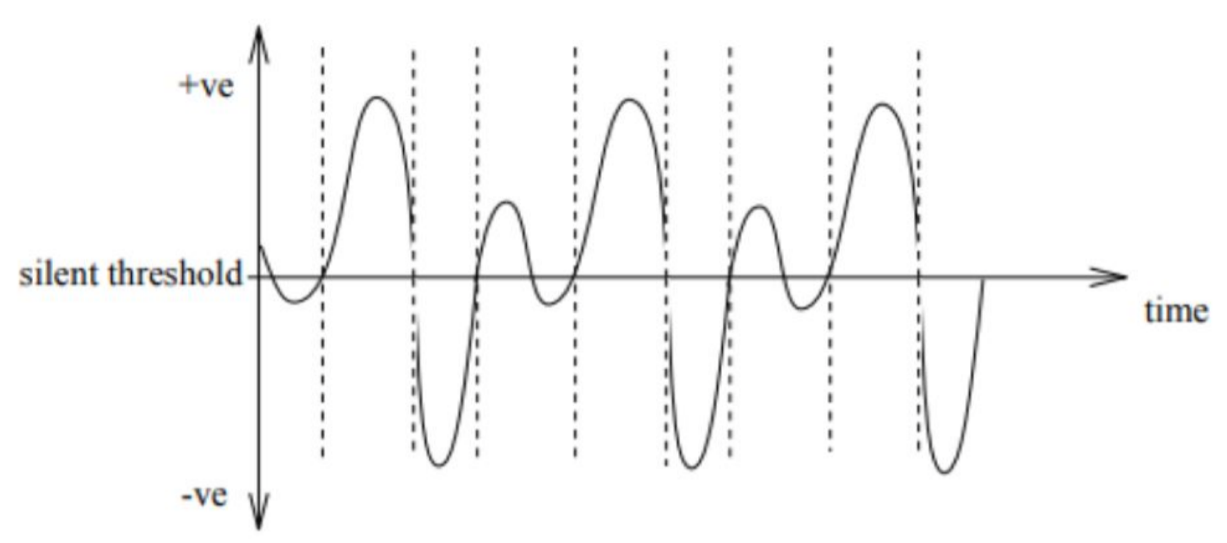
\includegraphics[width=0.5\textwidth]{Figures/zcr.png}
        \caption[An example signal with zero-crossings marked in dotted lines]{An example signal with zero-crossings marked in dotted lines\footnotemark{}}
    \end{figure}
    \footnotetext{Daoo, R. (2020, May 20). Algorithmic frequency/pitch detection series - part 1: Making a simple pitch tracker using zero... Medium. Retrieved May 14, 2022, from https://medium.com/the-seekers-project/algorithmic-frequency-pitch-detection-series-part-1-making-a-simple-pitch-tracker-using-zero-9991327897a4}
    \item \textbf{Harmonic Product Spectrum (HPS) (frequency domain)}\\
    As aforementioned, the human voice is not of pure tone. A musical note sung will consist of a series of peaks in its frequency spectrum. The peaks correspond to $f_0$ with other peaks indicating the harmonic components of integer multiples of $f_0$. 
    Exploiting this fact, the HPS algorithm creates multiple downsampled signal spectrums and compares them with the original spectrum, as shown in 
    \cref{HPS}\footnote{QLH Andre, I Khelf, Q Leclere. (2017). Harmonic product spectrum revisited and adapted for rotating machine monitoring based on IAS}.
    The strongest harmonic peak will line up no matter how many times we compress the spectrum.
    
    \begin{figure}[h]
        \centering
        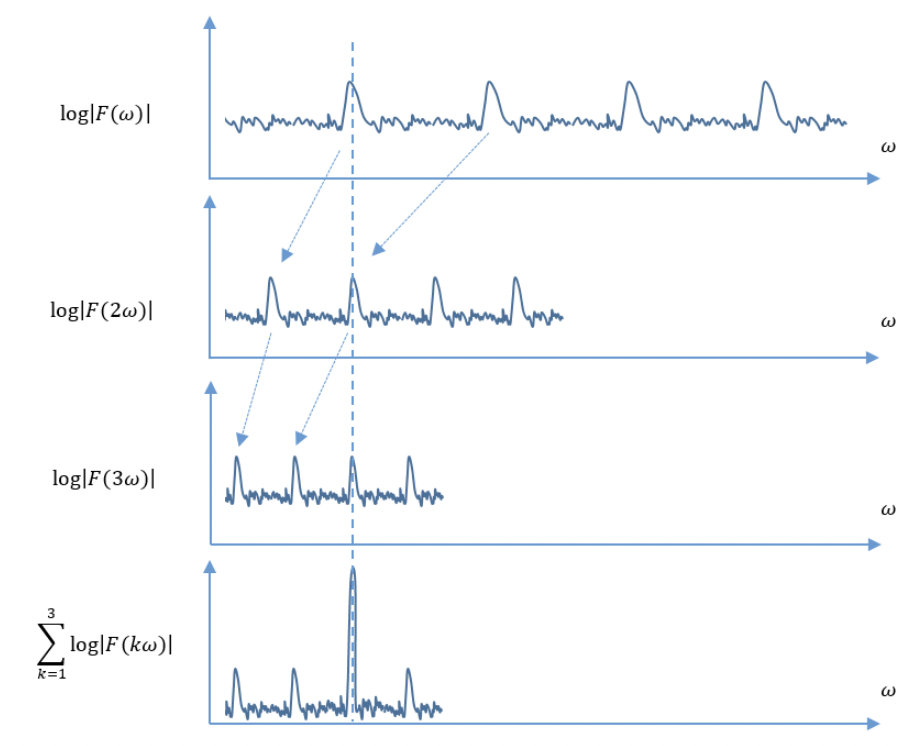
\includegraphics[width=0.5\textwidth]{Figures/HPS.png}
        \caption{Harmonically compressed log spectra}
        \label{HPS}
    \end{figure}
    
    Firstly, we convolve the signal with a Hanning window to segment the input:
    \[w(n) = \frac{1+cos(2\pi n/N-1)}{2}, \text{ for } 0 \leq n \leq N-1\] where $N$ is the number of samples.\\
    We then convert it from time-domain to frequency-domain by computing the short-time Fourier Transform:
    \[STFT \{x[n]\}(k,\omega) = X(k,\omega )= \sum _{n=-\infty }^{\infty }x[n]w[n-k]e^{-j\omega n}\]
    Lastly we compute the product of spectrum at harmonics of various frequencies and $f_0$ is estimated by:
    \[f_0 = argmax\prod_{k=1}^{n}|X(kf)|\] 

    \item \textbf{YIN algorithm/ autocorrelation (time domain)}\\
    As outlined by \cite{yin}, YIN algorithm is based on a slightly altered autocorrelation method:
    \[r_t(\tau)=\sum_{j=t+1}^{t+W-\tau}x_j x_{j+\tau}\]
    where $r_t(\tau)$ is the autocorrelation function (ACF) of lag $\tau$ calculated at time index $t$, $W$ is the integration
    window size. Note that as $\tau$ increases, $W$ decreases and the envelope of the function decreases, as shown in figure 
    \cref{taped}.

    \begin{figure}
        \centering
        \begin{subfigure}{.3\textwidth}
          \centering
          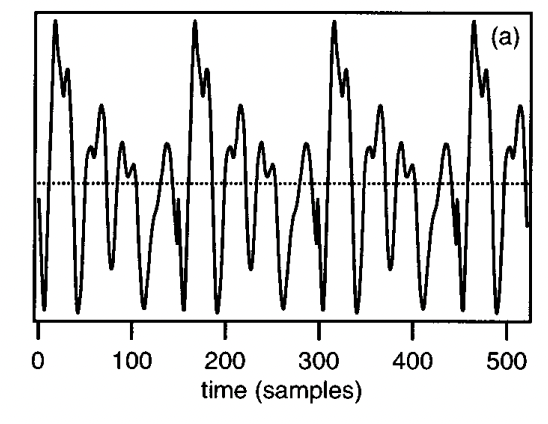
\includegraphics[width=1\linewidth]{Figures/signalwaveform.png}
          \caption{Signal waveform}
          \label{signal}
        \end{subfigure}%
        \begin{subfigure}{.3\textwidth}
            \centering
            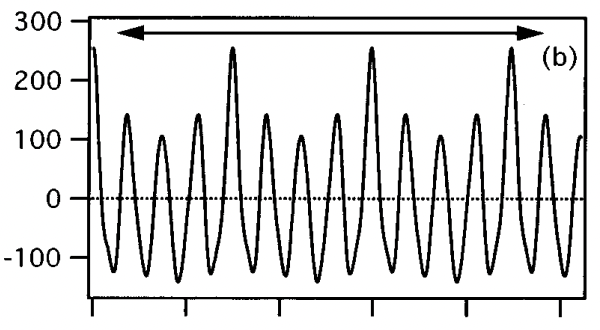
\includegraphics[width=1\linewidth]{Figures/acf.png}
            \caption{$r_t(\tau)$ calculated from \\ \cref{signal} using normal ACF}
            \label{acf}
          \end{subfigure}%
        \begin{subfigure}{.3\textwidth}
          \centering
          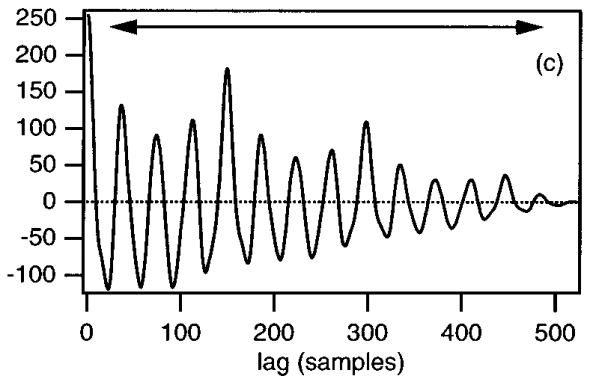
\includegraphics[width=1\linewidth]{Figures/taperedacf.png}
          \caption{$r_t(\tau)$ calculated with \\ \cref{CMNDF}}
          \label{taped}
        \end{subfigure}%
        \label{YIN}
    \end{figure}
    
    We then select the highest peak by exhaustive search within a user-defined range of lags; the corresponding time lag will be
    the inverse of our estimated $f_0$.

    To improve the error rates and target periodicity, de Cheveigné \& Kawahara introduced a cumulative mean normalized difference function (CMNDF)
    to replace ACF. 
    \begin{equation}
        \label{CMNDF}
        CMNDF(\tau) = \begin{cases}
             1                                              & \text{if $\tau = 0$} \\ 
            \frac{DF(\tau)}{(1/\tau)\sum_{j=1}{\tau} DF(j)} & \text{otherwise.}
        \end{cases}
    \end{equation}
    
    We then find $\tau$ that minimises $CMNDF(\tau)$ and the corresponding $f_0$.
    \label{sec:crepe}
    \item \textbf{CREPE (Convolutional Representation for Pitch Estimation) (Machine learning method)}\\
    CREPE is a data-driven algorithm developed by \cite{crepepaper} that operates directly on the time domain.
    It consists of a deep convolutional neural network (CNN) trained by synthesised audio from the RWC Music Database \footnote{Goto, Masataka and Oka. (Oct 2002). from https://staff.aist.go.jp/m.goto/RWC-MDB/}
    and MedleyDB \footnote{Bittner, R., Wilkins, J., Yip, H., \& Bello, J. (2016). MedleyDB 2.0: New Data and a System for Sustainable Data Collection. New York, NY, USA: International Conference on Music Information Retrieval (ISMIR\-16).}. 

    CNN is often seen in image-processing applications and is a network that uses convolution instead of the typical matrix multiplication.
    It consists of an input layer, hidden layers and an output layer. Hidden layers include convolution layers, pooling layers and fully connected layers.
    
    As shown in \cref{CREPE}, there are six hidden layers, and each layer is followed by a dropout layer with a dropout probability of 0.25. 

    Convolution layers are the building blocks of CNN since it performs feature extraction through convolution and activation functions like $ReLU$.
    Two hyperparameters defining a convolution operation are the kernel size and the number of kernels. Kernels in the convolutional layer context are convolutional
    filters. Hence, kernel size refers to the size of the filter mask, and the number of kernels relates to the number of output features desired. \cref{CREPE} shows the hyperparameters
    used in CREPE.

    Max pooling is often used in the operation of the pooling layer and is the operation used in CREPE. It outputs the maximum value in a patch extracted from the
    input tensor and discards the non-maximum values. 
    One advantage of using max-pooling is that it suppresses noise better than other dimensionality reduction methods like average pooling.

    A fully connected layer maps all extracted features in one layer to every activation unit of the next layer. In the context of CNN, it is often seen in the
    last few layers to compile the features for final output.

    \begin{figure}
        \centering
        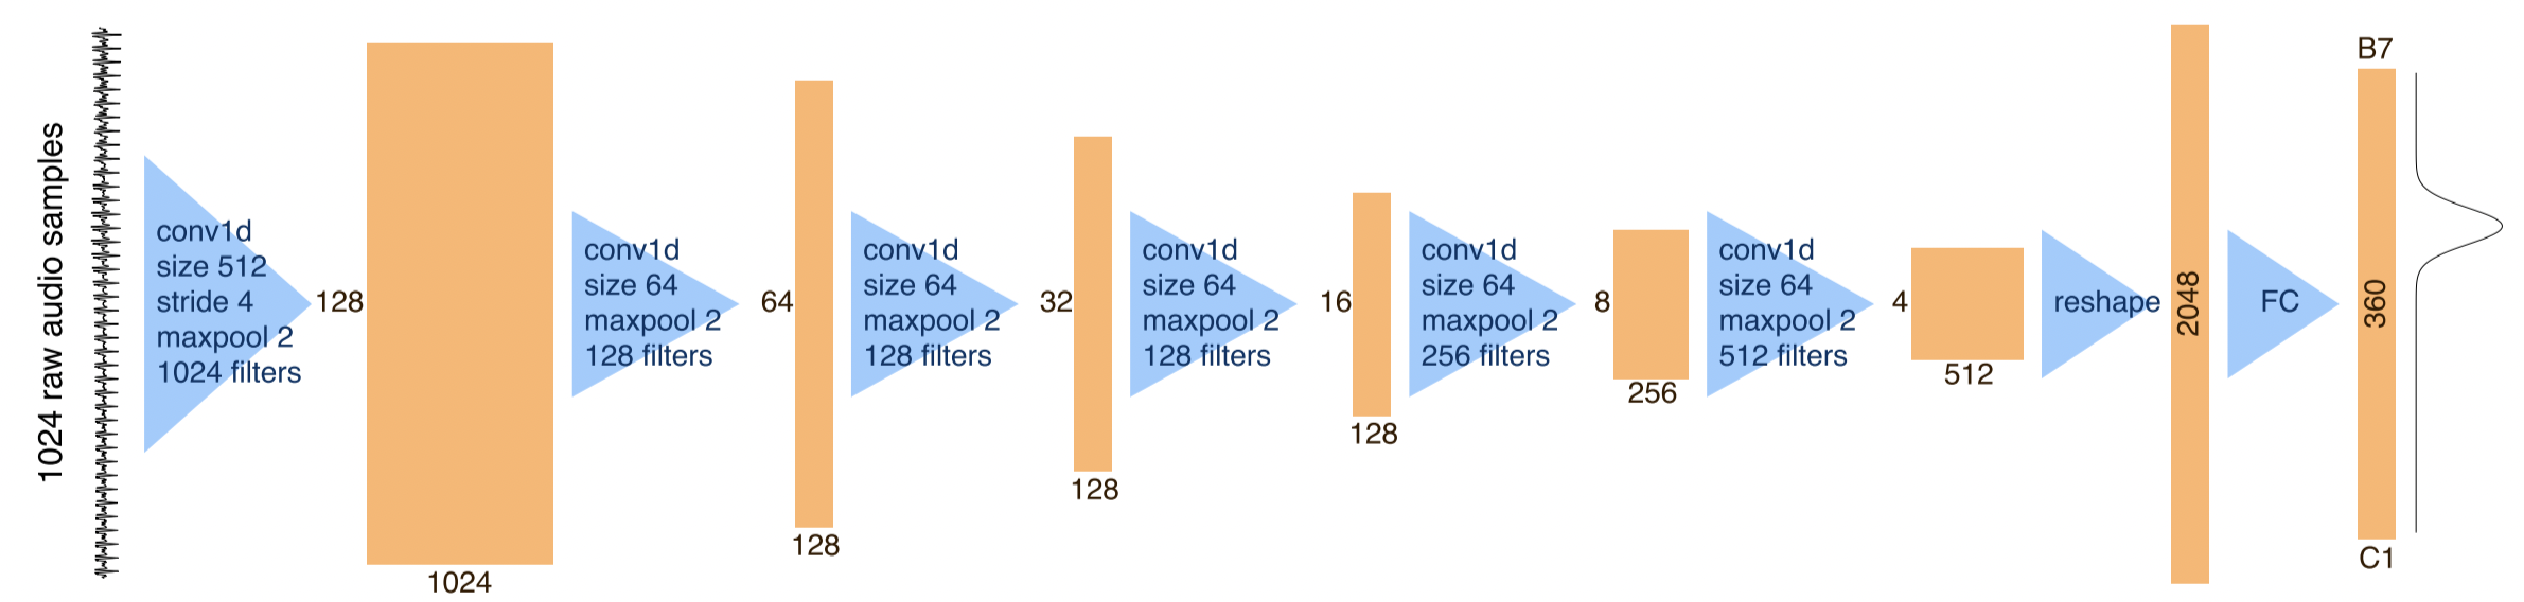
\includegraphics[width=0.85\columnwidth]{Figures/CREPE.png}
        \caption{The architecture of the CREPE algorithm}
        \label{CREPE}
    \end{figure}
\end{enumerate}

%-----------------------------------
%   SUBSECTION 2
%-----------------------------------
\subsection{Comparison between models and implementation}
Time-domain models are more intuitive and easier to understand when compared to frequency domain models.
Also, the time-domain implementation often takes up less computational resources and time.
In exchange, frequency-domain models are less sensitive to noise and perform well on polyphonic singings.

The zero crossings method will not be considered though it has the cheapest computational cost. One limitation is that
the threshold is fixed at 0, making it susceptible to noise and the vocal timbre of the user. Moreover, the method heavily assumes that the input audio is of pure tone, but unlike a tuning fork, the human voice is not a pure tone. It is 
composed of a fundamental frequency and upper harmonics\footnote{Encyclopædia Britannica, inc. (n.d.). Harmonic structure. Encyclopædia Britannica. Retrieved May 15, 2022, from https://www.britannica.com/topic/speech-language/Harmonic-structure }.  
This characteristic makes this method extremely unreliable.

Like the zero-crossings method, HPS is intuitive and has a low computational cost. But since it builds on the characteristics 
that the signal contains amplitudes at harmonics, if the input signal does not have sufficient magnitudes at other harmonics, the 
performance of HPS will suffer. Moreover, the resolution of the method depends on the length of the short-time Fourier Transform, which
determines the number of discrete frequencies that we can consider. But if we want a higher resolution and less graininess in our 
pitch output, more time is needed to perform the transform.

YIN has more satisfactory performance, but when the pitch varies rapidly (for example, if the user has a breathy timbre), it cannot 
estimate the pitch correctly as the algorithm uses a constant threshold. On the other hand, Kim et al. mentioned CREPE has a higher 
tolerance for inputs with different timbres since CREPE is trained with MedleyDB, which contains recordings of heterogeneous timbres. Figure 
\cref{CREPEperf} concludes the Raw Pitch Accuracy and Raw Chroma Accuracy for CREPE and other 2 PDA by Kim et al., and we will choose CREPE 
to implement in our model.

\begin{figure}[h]
	\centering
	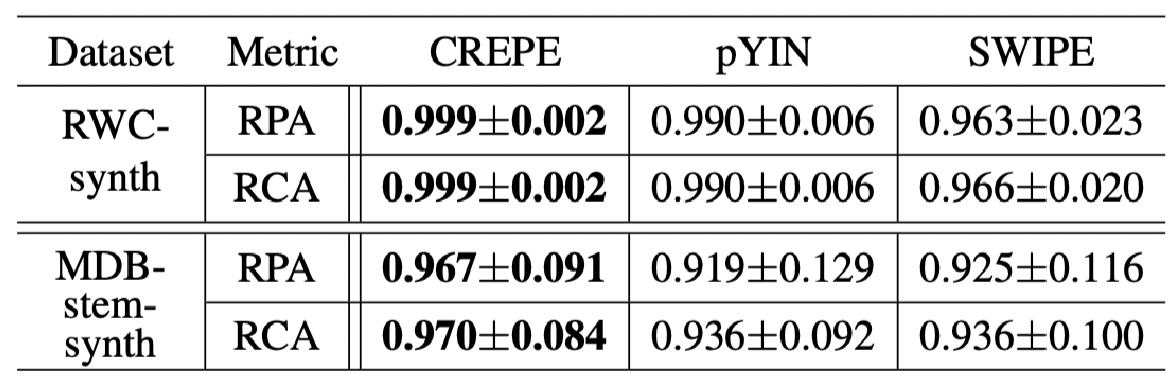
\includegraphics[width=0.8\columnwidth]{Figures/CREPEperf.png}
	\caption{Raw Pitch Accuracy and Raw Chroma Accuracy with the standard deviations for the 3 PDA tested by Kim et al.}
	\label{CREPEperf}
\end{figure}

The CREPE code uploaded by Kim et al. takes in the samples $y$, sampling rate $sr$ and a boolean parameter (True/ False) for Viterbi, a smoothing algorithm. 
It calculates pitch every 10 ms and outputs the timestamp, estimated frequency $\hat{f_0}$, confidence $c$ and an activation matrix for visualisation of outputs. 

The sampling rate of training data used by CREPE is at 16 kHz; thus, our input audio will need to be resampled to 16 kHz if the original $sr \neq 16 kHz$. If the user is using the iPhone 
built-in microphone to record, we need to set the preferred sampling rate to 16 kHz \footnote{Apple Inc. (2017, September). Audio Session Programming Guide. Configuring Device Hardware. Retrieved May 15, 2022, from https://developer.apple.com/library/archive/documentation/Audio/Conceptual/AudioSessionProgrammingGuide/OptimizingForDeviceHardware/OptimizingForDeviceHardware.html }
when coding for our iOS app.

One thing to note is that the algorithm centres the first frame at $t=0$ instead of starting the first frame at $t=0$ to avoid misalignment.

Continuing from the noise filtered signal, we use \emph{[y, sr]= scipy.io.wavfile.read(filename, mmap=False)} function to read the input and feed $[y, sr]$ 
into \emph{crepe.predict(y, sr, viterbi=True)}.
The output will be of the form [timestamp, $\hat{f_0}$, $c$, activation matrix].

We then manipulate the $\hat{f_0}$ array such that
\begin{equation}
    \hat{f_0}= 
\begin{cases}
    \hat{f_0},      & \text{if } c\geq 0.5\\
    0,              & \text{otherwise}
\end{cases}
\label{creperesult}
\end{equation}

In order to output the predicted frequencies as notes, we need to prepare a dictionary of notes with its corresponding frequencies, i.e. 
\emph{notesdict = {"A4": 440, "A\#4": 466.16, "B4": 493.88,...}}
and map the predicted frequency to the closest frequency that corresponds to a note with \emph{min(notesdict.items(), key=lambda (\_, freq): abs(freq - $f_0$))}
 
Finally, to target notes that lasted less than 10 timeframes (0.1s) (since they are likely to be misinterpreted/ noisy notes),
we neglect the misinterpreted note and add half of its duration to the frequency in front and behind respectively, i.e.
\begin{equation}
    T_{i-1} = T_{i-1} + \frac{T_i}{2}
        \quad \mathrm{and} \quad
    T_{i+1} = T_{i+1} + \frac{T_i}{2}
\end{equation}
Where $T_i$ represents the duration of the $i$th frequency.

From the implementation, we obtain \emph{note} and \emph{note\_duration} to pass to the data processor in \cref{data processor}.

%-----------------------------------
%   SUBSECTION 3
%-----------------------------------
\subsection{Improvements}

On top of the convolutional neural network model, we can integrate Maximum a Posteriori (MAP) estimation to improve the model.

Bayes' rule states: 
\[P(A\mid B)=\frac {P(B\mid A)P(A)}{P(B)}\]
where $P(A\mid B)$ is the posterior probability or the updated probability considering the evidence.\\
$P(B\mid A)$ is the likelihood, which is the probability of observing the evidence given the event has happened.\\
$P(A)$ is the prior probability, which is the probability before considering the evidence.\\
$P(B)$ is known as the marginal probability, which is the probability of an event irrespective of the outcomes of any evidence.

After dropping the denominator term $P(B)$ since it is a normalization constant, we come up with the following equation:
\[f_0 = \argmax_{f_0} P({f_0}\mid D) = \argmax_{f_0} P(D\mid {f_0}) P({f_0})\]
where D is the previous data, $f_0$ is the desired frequency, $P({f_0})$ is the prior computed by the CREPE model and $P(D\mid {f_0})$ is the likelihood
of observing the previous audio frequencies for a given frequency $f_0$.

With enough audio samples sung by the user, we can collect the frequencies they have sung. Then we can model the probability 
distribution $P(D\mid {f_0})$ as a Gaussian distribution in which the mean and variance are updated when observing a frequency given the previous audio samples. 

For instance, given the prior that a user is a bass singer (the lowest vocal range of all voice types), his inputs are around the low frequency. 
If the CREPE model wrongly predicts that he has sung a note of high frequency, the MAP estimate will reduce the probability that the output frequency is a high
frequency since our prior hints a low probability of that.
%----------------------------------------------------------------------------------------
%   SECTION 3
%----------------------------------------------------------------------------------------
\section{Key Detection Algorithm (KDA)}
\label{sec:KDA}
Other than detecting the pitch/ note of the input audio, it is also necessary to estimate the key of the music to aid the identification
of chords with the machine learning model in the later step.

From a music theory point of view, the most intuitive method to identify the key of a piece is to look at the key signature, which contains the number of sharps/ flats
in a piece, and the number defines which key the piece is in. But since our app targets amateurs, we will not expect them to be able to know what key will they be singing
in.

Krumhansl-Schmuckler algorithm (template-based) \footnote{Krumhansl, C. L. (2001). Cognitive Foundations of musical pitch. Oxford Univ. Press.} is an experimentally measured
tonal hierarchy is introduced by \cite{templatedata}, which contains 24 tonal profiles for major and minor keys in total. 

Each of the profiles contains 12 values which correspond to 12 notes in an octave. The values were obtained from the experiment where they asked the listeners to judge how well
a note fits in a key on a scale from 1 to 7 (1 stands for very bad, 7 stands for very good). 

\begin{figure}
    \centering
    \begin{subfigure}{.45\textwidth}
      \centering
      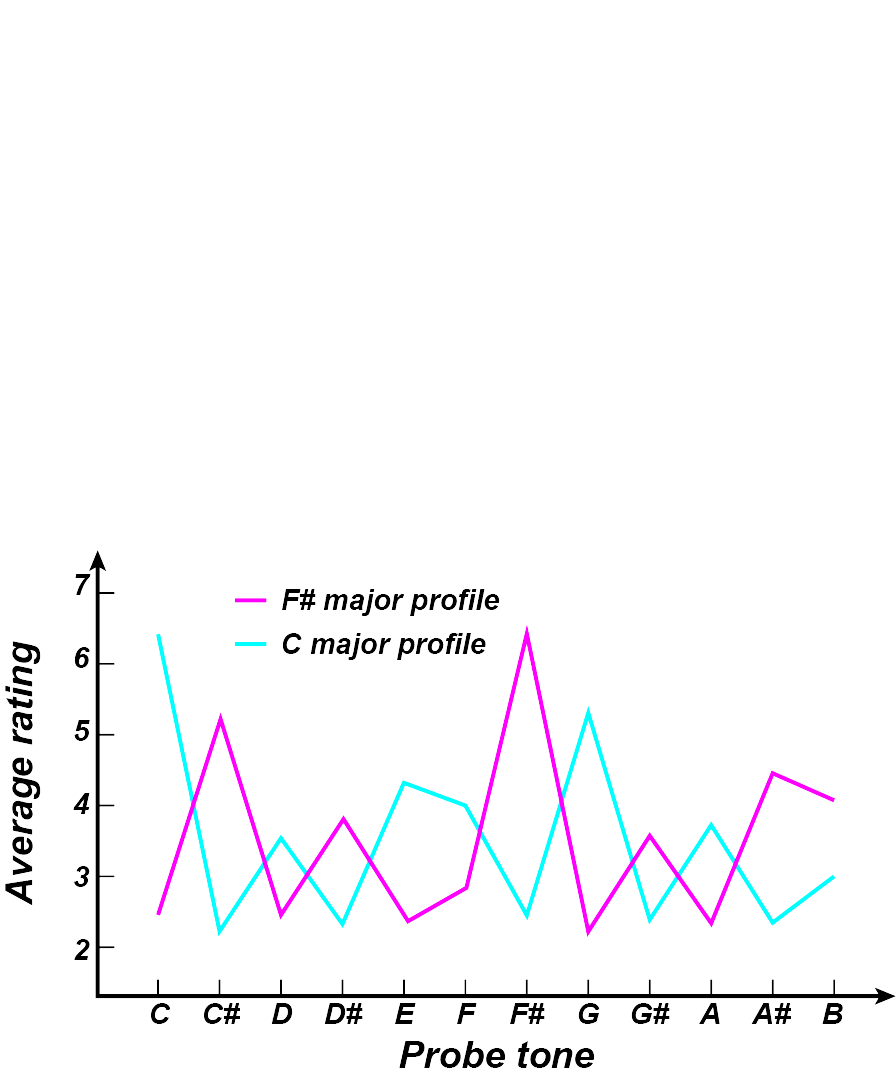
\includegraphics[width=1\linewidth,height=50mm]{Figures/profiles.png}
      \caption{Probe tone rating for F\# and C major}
      \label{probetone}
    \end{subfigure}%
    \begin{subfigure}{.45\textwidth}
        \centering
        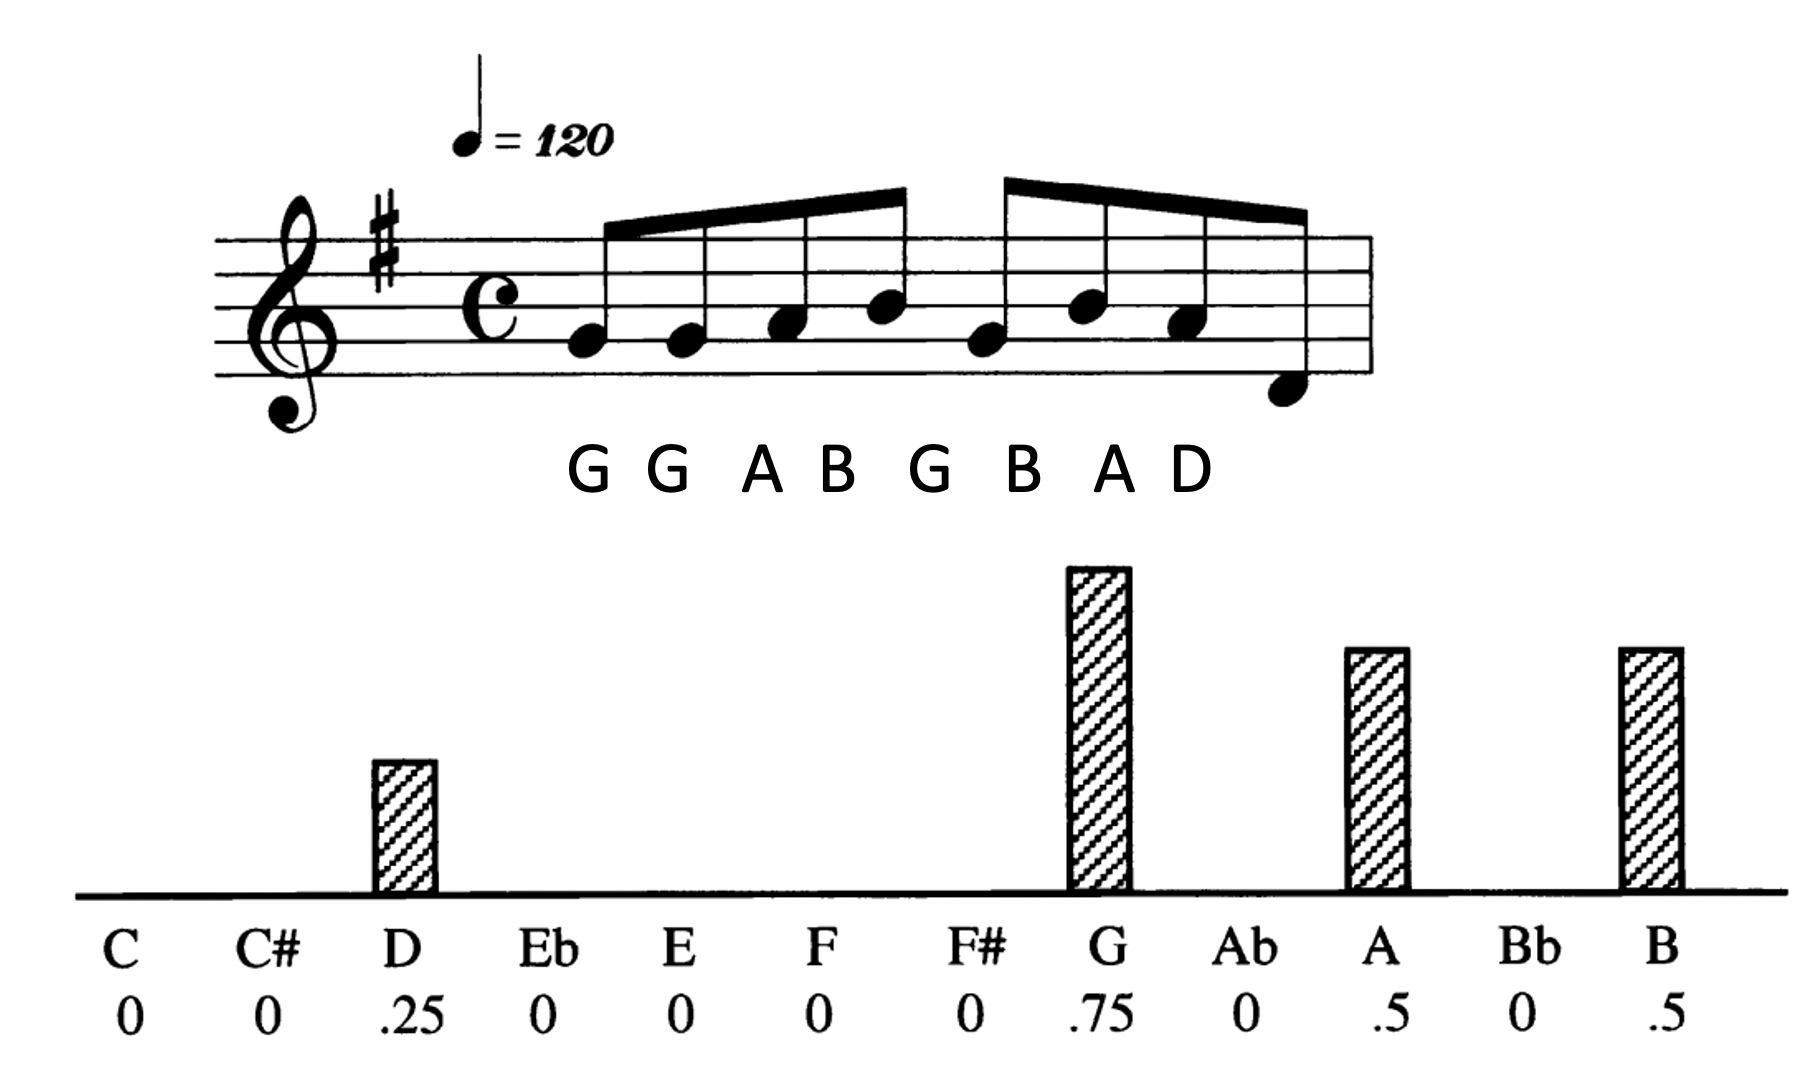
\includegraphics[width=1\linewidth,height=50mm]{Figures/inputvec.png}
        \caption{Input vector}
        \label{inputv}
      \end{subfigure}%
\end{figure}

\cref{probetone} serves as an example of the profiles, where sensibly, the base of the major has the highest rating (C has the highest rating in the C major profile, 
F\# sounds the best in the F\# major profile). 
Yet, one drawback is that the sense of key changes over time as affected by the evolution of music. While the method can still be utilised, the template will have to be
updated from time to time.

\subsection{Implementation}
Using the template from \cite{templatedata} in our model and it is represented as 24 vectors $\vec{P_{i,j}} \in \mathbb{R}^{12 \times 1}$, 
where $i$ is the tone of the profile, $j$ indicates whether the profile is in major or minor.
We also define the pitch class distribution (our input) as a vector $D \in \mathbb{R}^{12,1}$, where the 12 entries are the frequencies of the 12 notes that appeared in the audio.
$\vec{D}$ can be obtained by looping over the $\hat{f_0}$ array obtained in \cref{creperesult} and using the Python function \emph{collections.Counter([iterable-or-mapping])} to count the
number of occurrences. We then calculate the correlation between $\vec{P_{i,j}}$ and $\vec{D}$, which is essentially the dot product between the two.
\[ corr(\vec{P_{i,j}},\vec{D}) = \vec{P_{i,j}} \cdot \vec{D} \]
The estimated key ($i,j$) is found by looping over the 24 $\vec{P_{i,j}}$ vectors and finding the one that gives the maximum correlation.

As mentioned in \cref{data processor}, since the training dataset only contains songs in the major key to get accurate output, we have to assume our users sing in only
major keys (\cref{as:5}). Thus the $j$ component can be dropped, and we will pass the key \emph{i} to pass to the data processor.

%----------------------------------------------------------------------------------------
%   SECTION 4
%----------------------------------------------------------------------------------------
\section{Conclusion}
\label{sec:Summ}
In this chapter, we presented methodologies to filter noise, detect pitch and key. We will compile the strengths and weaknesses
in this section and \* mark represents the algorithm that we picked.
\begin{table}[h]
    \begin{tabular}{|lll|}
    \hline
    \multicolumn{1}{|l|}{Noise filter}                                                            & \multicolumn{1}{l|}{Strengths}                                                                                                                                                     & Limitations                                                                                                                                                                 \\ \hline
    \multicolumn{1}{|l|}{Low Pass Filter}                                                         & \multicolumn{1}{l|}{Easy and fast to implement}                                                                                                                                    & \begin{tabular}[c]{@{}l@{}}Cannot target broadband noise/\\ noise at low frequencies\\ Hard to set the cut-off frequency\\ for users in different environments\end{tabular} \\ \hline
    \multicolumn{1}{|l|}{\begin{tabular}[c]{@{}l@{}}Wavelet \\ Transform\end{tabular}}            & \multicolumn{1}{l|}{\begin{tabular}[c]{@{}l@{}}Based on both time and frequency\\ domain so localised information \\ about the signal can be efficiently \\ accessed\end{tabular}} & \begin{tabular}[c]{@{}l@{}}Sensitive to shifts in time\\ Poor directionality\\ Hard to set a mother wavelet\end{tabular}                                                    \\ \hline
    \multicolumn{1}{|l|}{\begin{tabular}[c]{@{}l@{}}Spectral \\ Reduction*\end{tabular}}          & \multicolumn{1}{l|}{\begin{tabular}[c]{@{}l@{}}Based on noise profile of the input \\ recording so it is more customized\end{tabular}}                                             & \begin{tabular}[c]{@{}l@{}}Requires user to input a noise \\ profile/ recording of the background\end{tabular}                                                              \\ \hline
    \multicolumn{3}{|l|}{}                                                                                                                                                                                                                                                                                                                                                                                                                                           \\ \hline
    \multicolumn{1}{|l|}{PDA}                                                                     & \multicolumn{1}{l|}{Strengths}                                                                                                                                                     & Limitations                                                                                                                                                                 \\ \hline
    \multicolumn{1}{|l|}{Zero crossing}                                                           & \multicolumn{1}{l|}{\begin{tabular}[c]{@{}l@{}}Intuitive\\ Cheapest to compute\end{tabular}}                                                                                       & \begin{tabular}[c]{@{}l@{}}Susceptible to noise and vocal \\ timbre\end{tabular}                                                                                            \\ \hline
    \multicolumn{1}{|l|}{\begin{tabular}[c]{@{}l@{}}Harmonic \\ Product \\ Spectrum\end{tabular}} & \multicolumn{1}{l|}{Low computational cost}                                                                                                                                        & \begin{tabular}[c]{@{}l@{}}Inaccurate if other harmonics do \\ not have a sufficient amplitude\\ Performance relies heavily on the \\ length of STFT\end{tabular}           \\ \hline
    \multicolumn{1}{|l|}{\begin{tabular}[c]{@{}l@{}}YIN/ \\ Autocorrelation\end{tabular}}         & \multicolumn{1}{l|}{\begin{tabular}[c]{@{}l@{}}Intuitive\\ Less susceptible to noise\end{tabular}}                                                                                 & \begin{tabular}[c]{@{}l@{}}Inflexible since it is based on a \\ constant threshold\end{tabular}                                                                             \\ \hline
    \multicolumn{1}{|l|}{CREPE*}                                                                  & \multicolumn{1}{l|}{\begin{tabular}[c]{@{}l@{}}Robust and tolerant to singing \\ with different timbres\end{tabular}}                                                              & \begin{tabular}[c]{@{}l@{}}Hard to interpret since it is a black \\ box model\end{tabular}                                                                                  \\ \hline
    \end{tabular}
\end{table}

We will pass \emph{note, note\_duration} from the PDA and \emph{key} to the data processor in \cref{data processor}.